%==============================================================================
% Three Measurable Failure Modes of Large Language Models
% Structure of the Error Distribution in Autoregressive Stochastic System
%
% Marek Hubka, Independent Researcher, Czech Republic
% May 2026
%==============================================================================
\documentclass[11pt,a4paper]{article}

\usepackage[utf8]{inputenc}
\usepackage[T1]{fontenc}
\usepackage{amsmath,amssymb,amsthm,mathtools}
\usepackage{geometry}
\usepackage{booktabs}
\usepackage{array}
\usepackage{xcolor}
\usepackage{graphicx}
\usepackage{hyperref}
\usepackage{enumitem}
\usepackage{float}
\usepackage{tikz}
\usepackage{pgfplots}
\usepackage{bm}
\usepackage{mdframed}
\usepackage{orcidlink}
\pgfplotsset{compat=1.18}
\usepgfplotslibrary{fillbetween, groupplots}
\usetikzlibrary{shapes, arrows.meta, positioning, calc,
                decorations.pathmorphing, decorations.pathreplacing}

\geometry{margin=1in}
\usepackage{todonotes}

\hypersetup{
  colorlinks=true,
  linkcolor=blue!70!black,
  citecolor=blue!60!black,
  urlcolor=blue!60!black
}

% -- Mode colours ---
\definecolor{mode1col}{RGB}{180,50,50}    % Mode 1 red
\definecolor{mode2col}{RGB}{50,80,180}    % Mode 2 blue
\definecolor{mode3col}{RGB}{50,180,80}    % Mode 3 green
\definecolor{neutral}{RGB}{128,128,128}
\definecolor{mode1bg}{RGB}{255,240,240}
\definecolor{mode2bg}{RGB}{232,240,255}
\definecolor{mode3bg}{RGB}{235,255,240}
\definecolor{insightbg}{RGB}{255,248,225}
\definecolor{insightcol}{RGB}{160,120,20}

% -- Theorem environments ---
\newtheorem{theorem}{Theorem}[section]
\newtheorem{lemma}[theorem]{Lemma}
\newtheorem{corollary}[theorem]{Corollary}
\newtheorem{proposition}[theorem]{Proposition}

% -- Macros ---
\newcommand{\Ccode}[3]{[\![#1,#2,#3]\!]}
\newcommand{\CS}{\mathsf{CS}}
\newcommand{\DE}{\mathsf{DE}}
\newcommand{\Hout}{\mathsf{H}_{\mathrm{out}}}
\newcommand{\srank}{\mathrm{srank}}
\newcommand{\Jbar}{\bar{J}}
\newcommand{\Norm}{\mathcal{N}}

%==============================================================================
\title{%
  \textbf{Three Measurable Failure Modes\\of Large Language Models}\\[0.5em]
  \large Structure of the Error Distribution in Autoregressive Stochastic System
}

\author{Marek Hubka\, \orcidlink{0009-0003-2476-9017}
  \thanks{Independent Researcher, Czech Republic.\\
    Email: \href{mailto:marek@tidesofuncertainty.com}{marek@tidesofuncertainty.com}}}

\date{May 2026}

\begin{document}
\maketitle

%==============================================================================
\begin{abstract}
The literature treats hallucination in large language models as a single phenomenon. We argue that there are three distinct failure modes. \emph{Autoregressive reinforcement} arises when a wrong token contaminates its own conditioning context, locking the model into a self-consistent but false trajectory. \emph{Confabulation} is fluent generation produced by parameter directions that received no training signal. \emph{Irreducible uncertainty} is the correct response of a calibrated probabilistic system to a genuinely ambiguous query. Each mode has a distinct cause, a distinct signature visible from outside the model, and a distinct class of effective remedies.

We give one quantitative metric per mode -- correction sensitivity ($\CS$), dimensional excess ($\DE$), and output entropy ($\Hout$). Underlying the three measurements is a single coding-theoretic construction, the syndrome table $S = \Norm(\Jbar \cdot V)^\top$, whose full derivation appears in the companion paper. A controlled synthetic model (deep-regime LSTM, $D = 256$, $L = 10$, six fixed seeds) empirically supports the framework end to end. The three metrics separate cleanly: $\CS$ exhibits a domain gap that narrows monotonically with the number of encoded knowledge domains from $0.273 \pm 0.095$ at $k = 1$ to $0.067 \pm 0.037$ at $k = 10$; $\DE$ rises monotonically; the Pearson correlation $r(\DE, \CS_{\mathrm{unknown}}) = 0.9896$ across $k$ predicts out-of-domain failure from weights alone. Causal localisation of an injected perturbation reaches $100\%$ over $180$ trials with a pre-injection/post-injection residual ratio of $\sim 2 \times 10^8$. Oracle correction is exact ($1.000000$ over $36{,}000$ trials); generic correction in a wrong direction worsens output by a factor of $1.76$--$5.21\times$ in expectation across $k$. A direct two-profile comparison at $N = 5$ and $N = 10$ shows that multicellular specialists win on Gram metrics while monolithic generalists win on identification -- the modular hierarchy is empirically justified, not assumed. The three failure modes are not bugs to be debugged. They are interference in a signal-propagating system, with mathematically necessary signatures and remedies matched to mechanism.

\medskip
\noindent\textbf{Keywords:} hallucination, autoregressive reinforcement, confabulation, syndrome measurement, dimensional excess, Jacobian variance, Gram metric, causal localisation, coding-theoretic bounds, language model reliability.
\end{abstract}

\tableofcontents
\bigskip

%==============================================================================
\section{Introduction}
\label{sec:intro}
%==============================================================================

A patient presenting with fever has not yet received a diagnosis. The fever is a symptom; the cause might be bacterial infection, viral infection, autoimmune disease, or heat stroke. Each cause demands a different treatment, and several treatments effective for one cause will harm a patient suffering from another. The first useful clinical step is differential diagnosis: deciding which of several distinct conditions is producing the symptom in front of you. Before that step, treatment is guessing.

``Hallucination'' in large language models (LLM) occupies precisely this position. The label has been applied to outputs that are incoherent, outputs that are fluent but invented, outputs that contradict their input, outputs that express overconfidence on ambiguous questions, and outputs whose only sin is that the user disagrees with them. These phenomena have different causes inside the model and respond to different interventions, yet a single word is used for all of them. The remedies most often deployed -- chain of thought, retrieval augmentation, temperature reduction, human feedback (RLHF) for calibration -- each address some of these phenomena and either leave the others untouched or actively make them worse.

This paper argues that LLM hallucination decomposes into three structurally distinct failure modes. Each mode arises from an independent property of stochastic system (hereafter: black box), has a measurable signature, and admits a different class of effective intervention. The modes interact, and the interaction is not symmetric: confabulation is a \emph{precondition} for autoregressive reinforcement on unknown domains, so the diagnostic order matters. Conflating the three under one label sends practitioners to remedies that target the wrong mechanism, and in the worst case to remedies that strictly worsen the output they were meant to repair.

\paragraph{Contributions.}
\begin{enumerate}[nosep]
    \item A taxonomy of three failure modes with distinct causal mechanisms derived from the geometric structure of the parameter space (\ref{sec:modes}).
    \item Three computable quantitative metrics, one per mode (\ref{sec:protocol}).
    \item The syndrome algebra framework: we state the root equation $S = \Norm(\Jbar \cdot V)^\top$ and three immediate consequences (\ref{sec:algebra}). The full derivation, the extension from the perfect quantum error correcting code~\cite{Laflamme1996, Bennett1996}, and all proofs are in the companion paper~\cite{SyndromeAlgebra}.
    \item Experimental validation on a synthetic controlled lstm2 model (six scripts, $k = 1, \ldots, 10$, six fixed seeds) supporting each prediction of the framework: the three metrics separate, $r(\DE, \CS_{\mathrm{unknown}}) = 0.9896$, causal localisation is exact, oracle correction is exact, and generic correction in a wrong direction is harmful by a factor of $1.76$--$5.21\times$ (\ref{sec:experiments}).
    \item Empirical justification of the modular hierarchy. A direct comparison of multicellular specialists against monolithic generalists at $N = 5$ and $N = 10$ shows the two architectures specialise for different diagnostic roles (\ref{sec:exp-modular}). The modular hierarchy is a theorem of the Singleton bound~\cite{Singleton1964, Ekert1996, SyndromeAlgebra} not an engineering preference.
\end{enumerate}

All measurements in this paper require access to weight matrices. The companion paper~\cite{SyndromeAlgebra} proves that the underlying construction is the unique extension of the discrete $\Ccode{5}{1}{3}$ quantum error-correcting code to the continuous real-valued regime.

The paper is organised as follows. Section~\ref{sec:motivation} motivates the stochastic framing and recounts the origin of the framework in quantum error-correcting codes. Section~\ref{sec:modes} defines the three modes and their interaction. Section~\ref{sec:algebra} states the syndrome algebra without proof. Section~\ref{sec:protocol} gives the measurement definitions. Section~\ref{sec:experiments} reports the experimental validation. Section~\ref{sec:pipeline} states the diagnostic pipeline and the Reliability Principle. Section~\ref{sec:predictions} lists eight predictions. Sections~\ref{sec:related}--\ref{sec:conclusion} discuss related work, scope, and open questions.


%==============================================================================
\section{Motivation}
\label{sec:motivation}
%==============================================================================

\subsection{The probabilistic lens}
\label{sec:mot-prob}

A language model is a stochastic system (the black box). Its output is a probability distribution over continuations of the input prefix, not a deterministic function of that prefix. The same prompt can yield different outputs across runs, across model instances, and across small perturbations of the input. Treating such a system as a deterministic program that occasionally malfunctions misframes the question. The deterministic question is ``why does the model sometimes get things wrong?'' The probabilistic question is sharper: \emph{what is the structure of the error distribution, and can it be characterised?}

This shift in framing changes what counts as an answer. A deterministic program either contains a bug or it does not. A stochastic system distributes its output over a set of possibilities, and that distribution has properties -- support, concentration, sensitivity to perturbation, mass on alternatives -- that are themselves measurable. Reliability becomes the question of how the output distribution responds when the model, the input, or the parameters change. Errors are not bugs in a program. They are properties of the distribution.


\subsection{Origin in quantum error-correcting codes}
\label{sec:mot-qecc}

The framework presented here arose from independent work in quantum information. In quantum error-correcting code (QECC)~\cite{NielsenChuang2000, Laflamme1996, Bennett1996} , an error is diagnosed via syndrome measurement: an ancilla observable is measured whose outcome is the image of the error under the parity-check matrix. The ancilla outcome identifies which error occurred without revealing or disturbing the encoded information. The diagnostic and the encoded data are decoupled by construction.

The author observed that LLM outputs are probabilistic in the same sense as quantum measurements: the system answers ``what is the next token?'' by sampling from a distribution, and a perturbation of the underlying system shifts that distribution rather than producing a deterministic output. The question arose: if a neural network's weight perturbations play the role of errors, and output-distribution changes play the role of syndrome observables, does the syndrome algebra transfer?

The $\Ccode{5}{1}{3}_2$ code was the anchor. Its parity-check matrix maps single-qubit error operators to four-bit syndromes; the construction has been the standard example of a perfect quantum code for thirty years. The generalisation required three replacements applied simultaneously: replace the Pauli error bases with the SVD directions $\{v_k\}$ of the weight matrix, replace the parity-check matrix with the averaged Jacobian $\Jbar$ of the logit map at probe inputs, and replace finite-field arithmetic over $\mathbb{F}_2$ with real-valued arithmetic over $\mathbb{R}$ via row-wise normalisation $\Norm$. Under these three substitutions the syndrome table becomes
\[
   S \;=\; \Norm(\Jbar \cdot V)^\top.
\]
The companion paper~\cite{SyndromeAlgebra} proves that this is the unique $q \to \infty$ limit of the discrete construction, that the $\Ccode{5}{1}{3}_2$ code is recovered as the binary special case at $q = 2$, and that the resulting algebra admits four immediate consequences governing measurement precision, correction guarantees, null space behaviour, and capacity-robustness trade-offs. The present paper takes those results as given and applies them to the diagnosis of LLM failure modes.

The insight this construction generated is the one that organises this paper. Hallucinations are not bugs. They are interference in a signal-propagating space: the same mathematical phenomenon as bit-flip errors in a noisy communication channel, now expressed in the weight-activation space of the black box. The \emph{shapes} of the interference -- self-consistent feedback, null-space emission, irreducible spread under ambiguity -- are mathematically necessary properties of any system of this kind. The syndrome algebra gives each a name and a measurement.


\subsection{Scope of the analogy}
\label{sec:mot-scope}

We do not claim that LLMs are quantum systems. We do not claim that quantum mechanics explains their behaviour. The analogy is structural: both systems exhibit a linear map from a perturbation space to an observable space, and both maps can be inverted to identify the perturbation that produced an observed change. The hypothesis was generated by quantum-mechanical intuition; its validation rests on differential geometry, spectral theory, and probability theory, applied to real-valued weight matrices and real-valued output distributions, without any quantum mechanical content. The $\Ccode{5}{1}{3}_2$ quantum code reappears in Section~\ref{sec:algebra} as the binary special case of a more general real-valued construction. Nothing in the experiments depends on quantum mechanics.


%==============================================================================
\section{The Three Failure Modes}
\label{sec:modes}
%==============================================================================

The three modes arise from three independent structural properties of any black box. They have different causes inside the model, different observable signatures, and different remedies. They are not three names for one phenomenon. Figure~\ref{fig:taxonomy} states the taxonomy at a glance.

\begin{figure}[H]
\centering
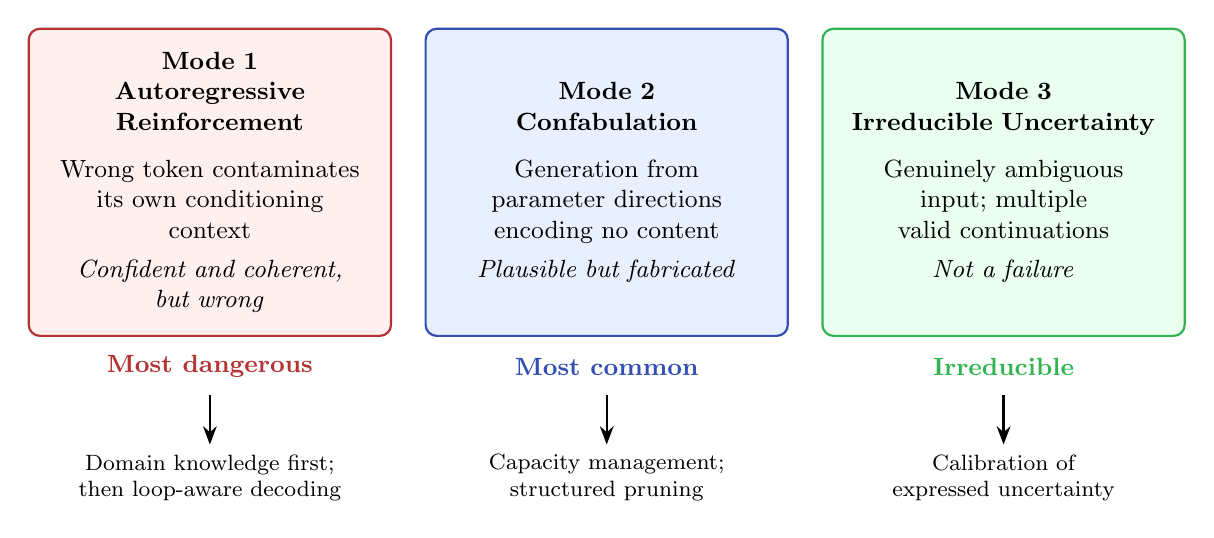
\begin{tikzpicture}[>=Stealth, scale=0.9,
    box/.style={draw, thick, rounded corners, minimum width=4.6cm,
                minimum height=3.9cm, text width=4.3cm, align=center,
                font=\small}]

    \node[box, fill=mode1bg, draw=mode1col] (m1) at (-5.6, 0) {
        \textbf{Mode 1}\\
        \textbf{Autoregressive Reinforcement}\\[6pt]
        Wrong token contaminates\\its own conditioning\\context\\[3pt]
        \textit{Confident and coherent,}\\
        \textit{but wrong}
    };

    \node[box, fill=mode2bg, draw=mode2col] (m2) at (0, 0) {
        \textbf{Mode 2}\\
        \textbf{Confabulation}\\[6pt]
        Generation from\\parameter directions\\encoding no content\\[3pt]
        \textit{Plausible but fabricated}
    };

    \node[box, fill=mode3bg, draw=mode3col] (m3) at (5.6, 0) {
        \textbf{Mode 3}\\
        \textbf{Irreducible Uncertainty}\\[6pt]
        Genuinely ambiguous\\input; multiple\\valid continuations\\[3pt]
        \textit{Not a failure}
    };

    \node[font=\bfseries\small, mode1col] at (-5.6, -2.6) {Most dangerous};
    \node[font=\bfseries\small, mode2col] at (0, -2.6) {Most common};
    \node[font=\bfseries\small, mode3col] at (5.6, -2.6) {Irreducible};

    \draw[->, thick] (-5.6, -3.0) -- (-5.6, -3.7)
        node[below, font=\footnotesize, text width=4.0cm, align=center]
        {Domain knowledge first;\\then loop-aware decoding};
    \draw[->, thick] (0, -3.0) -- (0, -3.7)
        node[below, font=\footnotesize, text width=4.0cm, align=center]
        {Capacity management;\\structured pruning};
    \draw[->, thick] (5.6, -3.0) -- (5.6, -3.7)
        node[below, font=\footnotesize, text width=4.0cm, align=center]
        {Calibration of\\expressed uncertainty};
\end{tikzpicture}
\caption{Three structurally distinct failure modes. Each has a different
mechanism, a different measurable signature, and a different intervention
class. Treating them as one phenomenon obscures the differential diagnosis.}
\label{fig:taxonomy}
\end{figure}


\subsection{Mode 1: Autoregressive Reinforcement}
\label{sec:mode1}

In autoregressive generation each output token enters the input prefix that conditions the next token. If the model emits a wrong token at position $t$, the prefix at position $t+1$ contains a falsehood. Conditioning on a prefix that contains a falsehood, the model selects the next token to be consistent with that falsehood. The mechanism that produced the error produces the cover-up.

The result is a feedback loop in which each step makes the next step more plausible and the original error harder to dislodge. The trajectory of generation drifts toward a fixed point that is internally coherent and externally false. This is the most dangerous of the three modes because the output exhibits no distributional signal of trouble: token-level entropy remains low, surface form remains fluent, and downstream consumers see a confident answer with the wrong content. The fixed-point attractor structure is formally analogous to the self-consistent causal loops of Novikov~\cite{Novikov1989}; we cite the formal analogy without claiming any physical correspondence.

The metric for Mode~1 is correction sensitivity ($\CS$): the mean distributional distance between corrupted and clean continuations over a fixed token horizon, measured in the model's own logit space. High $\CS$ means the injected error reshapes subsequent generation. Low $\CS$ means the model self-corrects.


\subsection{Mode 2: Confabulation}
\label{sec:mode2}

A weight matrix $W$ has a singular value decomposition $W = U \Sigma V^\top$ in which the right singular vectors $\{\mathbf{v}_k\}$ are an orthonormal basis of the input space. Training shapes only the directions whose singular values $\sigma_k$ are large: these are the signal space, the space of features the data have selected for. Directions with $\sigma_k \approx 0$ received no gradient signal during training. They form the null space of the layer's effective transformation, a set of parameter directions that the model can use to generate output but that encode no content in the technical sense.

On in-distribution inputs the null space is computationally invisible: its contribution to the output is negligible, and it cannot be distinguished from no perturbation at all. On out-of-distribution inputs the null space activates freely, because the orthogonality between signal and null directions is a property of the in-distribution manifold and need not hold elsewhere. Output produced through the null space is fluent -- because the \emph{surface form} of language is a learned signal-space property -- but empty in content, because the parameter directions producing the content were never shaped by training data. The model does not know that it does not know. By construction it cannot know.

The metric for Mode~2 is dimensional excess ($\DE$): the ratio of nominal input dimension to the stable rank of the weight matrix. $\DE \gg 1$ means the weight matrix uses far fewer effective directions than its parameter count suggests. The remaining nominal directions are the confabulation subspace.


\subsection{Mode 3: Irreducible Uncertainty}
\label{sec:mode3}

Some queries are genuinely ambiguous: they admit multiple correct continuations within the training distribution, or no clearly correct continuation at all. ``Will it rain tomorrow in this town?'' has no unique answer in a corpus that does not include tomorrow's weather. ``What is the right thing to do?'' has many answers across many ethical frameworks. \emph{The correct response} of a calibrated probabilistic system to such a query is high output entropy -- a distribution spread across many plausible answers, none favoured.

This is not a failure of the model. It is the model's correct acknowledgement of the input's underspecification. Treating it as a failure produces overconfidence on hard queries: a low-temperature output committed to one of many equally good answers, presented as if the others did not exist. Reducing temperature to suppress Mode~1 trajectories simultaneously suppresses Mode~3 calibration. The same parameter helps one mode and harms another.

The metric for Mode~3 is output entropy ($\Hout$): the entropy of the next-token distribution, or the diversity of stochastic draws under the same prompt. Diagnosis requires ground truth about the query, not only about the output: high $\Hout$ on a known-answer query is miscalibration, while high $\Hout$ on a genuinely ambiguous query is correct behaviour.


\subsection{The interaction}
\label{sec:interaction}

The three modes are independent in mechanism but not symmetric in their interaction. Mode~2 is a precondition for Mode~1 on unknown domains: the model cannot self-correct toward a correct trajectory it does not contain. When the relevant domain lies in the null space rather than the signal space, the only fixed points available are self-consistent wrong ones.

The empirical signature of this dependency is the monotone rise of the $\CS$ floor with $k$, the number of simultaneously encoded domains. The known-domain $\CS$ rises from $0.310$ at $k = 1$ to $0.811$ at $k = 10$ (\ref{sec:exp-modes}). As the model encodes more domains in a single parameter space, its per-domain attractor weakens proportionally: the Gram metric\footnote{We term $G = W^\top W$ the \emph{Gram metric} because it plays the role of a Riemannian metric on the parameter subspace spanned by the weight matrix $W$: it assigns a geometry to perturbation directions, with $\sigma_k^2 = v_k^\top G\, v_k$ giving the squared length of the $k$-th SVD direction. The term \emph{Gram matrix} refers to the same object in linear algebra; we adopt \emph{Gram metric} to emphasise its geometric role.} $G = W^\top W$ on the shared input space is a superposition of $k$ per-domain geometries, and interference among them raises the $\CS$ floor even on known queries. The pure specialist ($k = 1$) has the strongest attractor and the cleanest distinction between known and unknown. The generalist's attractor on any one domain is correspondingly weaker.

Simultaneously, the Pearson correlation $r(\DE, \CS_{\mathrm{unknown}}) = 0.9896$ across $k$ values: the null space size, measurable from weights alone without any test input, predicts out-of-domain failure severity at near-perfect linearity. This is the operational statement that Mode~2 is the precondition for Mode~1: a measurement made on the weights alone ($\DE$) predicts the failure that manifests at test time ($\CS$ on unknown queries), and the correlation is sharp.

The $\Hout$ ratio shows a different pattern: an inverted-U rising from $26.85\times$ at $k = 1$ to a peak of $202.66\times$ at $k = 5$, then falling to $176.52\times$ at $k = 10$. Mode~3 is sharpened by inter-domain contrast -- a model that has encoded several distinct domains becomes a sharper anomaly detector across them, raising the ratio of out-of-domain to in-domain entropy. Beyond a certain capacity, the single output distribution must accommodate too many distinct domains and the contrast begins to compress. The inverted-U peak at $k = 5$ is the empirical operating point of this trade-off in the lstm2 architecture.

The diagnostic order follows. Architectural interventions that target the feedback loop -- contrastive decoding, self-consistency rerolls, loop-aware sampling -- cannot succeed on a domain the model does not know, because there is no correct trajectory for the loop to converge to. The remedy for Mode~1 on unknown domains is not architectural; it is the supply of the missing knowledge whose absence created the degenerate fixed point. Mode~2 must be measured before Mode~1.


%==============================================================================
\section{The Syndrome Algebra}
\label{sec:algebra}
%==============================================================================

This section states the mathematical object used in the rest of the paper. The full derivation, the $q \to \infty$ limit theorem, the $\Ccode{5}{1}{3}_2$ recovery, and the proofs of all consequences are in~\cite{SyndromeAlgebra}. The present paper uses the algebra; it does not re-derive it.

\subsection{The root equation}
\label{sec:algebra-root}

Let $W \in \mathbb{R}^{d_{\mathrm{out}} \times d_{\mathrm{in}}}$ be a weight matrix with singular value decomposition $W = U \Sigma V^\top$, and let $\ell(x; W) \in \mathbb{R}^q$ be a logit map taking input $x \in \mathbb{R}^{d_{\mathrm{in}}}$ to $q$-dimensional output logits. Consider a rank-one SVD-aligned perturbation in direction $k$,
\[
   \Delta W_k(\varepsilon) \;=\; \varepsilon\, u_k v_k^\top
   \;\in\; \mathbb{R}^{d_{\mathrm{out}} \times d_{\mathrm{in}}}.
\]
The first-order change in the logit at probe input $x_i$ is $\delta_k(x_i, \varepsilon) = \varepsilon\, J(x_i)\, v_k + O(\varepsilon^2)$, where $J(x_i) \in \mathbb{R}^{q \times d_{\mathrm{in}}}$ is the logit Jacobian. Averaging over $n_p$ probe inputs and normalising row-wise gives the dictionary syndrome
\[
   s_k \;=\; \Norm\bigl(\bar\delta_k\bigr)
         \;=\; \Norm\bigl(\Jbar\, v_k\bigr) \in \mathbb{R}^q,
   \quad \|s_k\| = 1,
\]
where $\Jbar = n_p^{-1} \sum_i J(x_i)$ is the averaged Jacobian and $\Norm(w) = w/\|w\|$ is $\ell_2$ normalisation. Stacking the $r$ rows gives the syndrome table:
\begin{equation}
\label{eq:syndrome}
\boxed{\;
   S \;=\; \Norm(\Jbar \cdot V)^\top
   \;\in\; \mathbb{R}^{r \times q}.
\;}
\end{equation}
Row $k$ of $S$ is the syndrome $s_k$ of the $k$-th SVD direction.

\paragraph{Three-line sketch.} The Taylor expansion of $\ell$ around $W$ gives $\delta_k(x, \varepsilon) = \varepsilon\, J(x)\, v_k + O(\varepsilon^2)$. Averaging the linear term over probe inputs and dividing by $\varepsilon$ yields $\Jbar\, v_k$; row-wise normalisation is the continuous analogue of taking residues mod $q$ in the discrete code. Full derivation, proof of the $q \to \infty$ limit, and the explicit reduction to the $\Ccode{5}{1}{3}_2$ code by setting $q = 2$, $\Jbar \leftrightarrow H$ (parity-check matrix mod $2$), and $V \leftrightarrow I_{10}$ (Pauli basis in symplectic representation) appear in~\cite{SyndromeAlgebra}.


\subsection{Three consequences}
\label{sec:algebra-thms}

Three properties of the syndrome table support every empirical claim in this paper. 

\begin{theorem}[Oracle correction is exact]
\label{thm:oracle}
Let $W$ be perturbed by $\Delta W_k(\varepsilon) = \varepsilon\, u_k v_k^\top$. If the direction $k$ and magnitude $\varepsilon$ are identified, the inverse perturbation restores $W$ exactly:
\[
   W_{\mathrm{corrected}}
   \;=\; W + \varepsilon u_k v_k^\top - \varepsilon u_k v_k^\top
   \;=\; W,
\]
so the corrected logit equals the original on every input. The residual is zero, not small.
\end{theorem}

\begin{theorem}[Crossing error is positive in expectation]
\label{thm:cross}
Let the true perturbation be in direction $k$ but the inverse correction be applied in direction $j \neq k$. Under the averaged Jacobian $\Jbar$ and the orthogonality $\langle v_j, v_k \rangle = 0$, the expected squared output residual after correction strictly exceeds the residual before correction:
\[
   \mathbb{E}\bigl[\|\delta_{\mathrm{wrong}}\|^2\bigr]
   \;>\;
   \mathbb{E}\bigl[\|\delta_{\mathrm{perturbed}}\|^2\bigr].
\]
\emph{Scope.} The inequality holds for the averaged Jacobian and is exact on the linear path. Per-input violations occur when the local Jacobian $J(x)$ deviates substantially from $\Jbar$. The deviation is quantified by the per-direction Jacobian variance $V_j = n_p^{-1} \sum_i \|J(x_i) v_j -
\Jbar v_j\|^2$. The Jacobian Uncertainty Principle (JUP, Theorem~5 in~\cite{SyndromeAlgebra}) gives the irreducible bound on per-input violations.
\end{theorem}

\begin{theorem}[Null space is the confabulation subspace]
\label{thm:null}
For SVD directions $v_k$ with $\sigma_k \to 0$:
\begin{itemize}[nosep]
  \item On in-distribution inputs, the syndrome norm $\|\Jbar v_k\| \to 0$. The direction is computationally invisible: it contributes nothing to the model's behaviour on the training manifold.
  \item On out-of-distribution inputs, $\|\Jbar v_k\|$ is unconstrained. The direction is free to contribute to generation, producing fluent output (surface form is a learned signal-space property) whose content is unconstrained by training data.
\end{itemize}
The collection of small-$\sigma$ directions is the confabulation subspace; $\DE = d_{\mathrm{in}} / \srank(W)$ measures its size.
\end{theorem}

\begin{corollary}[$k = 1$ specialist saturates the Singleton bound]
\label{fix:cor1}
A model trained on $k = 1$ domain achieves the maximum Singleton distance $d = n$ on that domain. A model trained on $k$ domains satisfies $d \leq n - k + 1$, so per-domain distance falls by one for each additional domain encoded in the shared parameter space. The $k = 1$ specialist is therefore the architectural optimum for per-domain reliability, and the multicellular hierarchy of $K$ separate $k = 1$ cells dominates a single $k = K$ generalist by $K - 1$ in achievable distance per domain. Proof: in~\cite{SyndromeAlgebra}.
\end{corollary}
 
\begin{corollary}[Fine-tuned specialists cannot achieve Singleton distance]
\label{fix:cor2}
Let $W_0$ be a weight matrix pretrained on $K$ domains, with null space $\Norm(W_0) = \mathrm{span}\{v_k : \sigma_k(W_0) \approx 0\}$, and let $W_1$ be obtained from $W_0$ by fine-tuning on a single target domain. Fine-tuning gradients vanish in null-space directions by construction: for $v_k \in \Norm(W_0)$, the activation through direction $v_k$ is zero throughout pretraining, so the fine-tuning loss has no curvature along $v_k$ and the gradient component $\nabla_W \mathcal{L} \cdot v_k$ is zero at every fine-tuning step. Therefore $\Norm(W_0) \subseteq \Norm(W_1)$: the inherited null space persists. The effective domain count of $W_1$ remains $\geq K$, and the maximum achievable Singleton distance is bounded by $d \leq n - K + 1$, not $n$. A scratch-trained $k = 1$ specialist is required for the $d = n$ bound. Proof: in~\cite{SyndromeAlgebra}.
\end{corollary}

\paragraph{The $\Ccode{5}{1}{3}_2$ correspondence.} The standard $\Ccode{5}{1}{3}_2$ quantum error-correcting code is recovered from \eqref{eq:syndrome} by three substitutions: $q = 2$, $\Jbar \leftarrow H$ (parity-check matrix mod $2$), and $V \leftarrow I_{10}$ (Pauli basis in the standard symplectic representation). Under these substitutions $S =
H^\top \pmod 2$, the standard four-bit syndrome lookup table for the fifteen single-qubit errors and the identity. The complete correspondence table and worked example are in Appendix~A of~\cite{SyndromeAlgebra}.


%==============================================================================
\section{Measurement Protocol}
\label{sec:protocol}
%==============================================================================

All three modes are individually measurable given access to the model's weight matrices. One metric per mode.


\subsection{Correction sensitivity (Mode 1)}
\label{sec:protocol-cs}

Correction sensitivity quantifies the propagation of an injected error through subsequent generation:
\begin{equation}
\label{eq:cs}
\CS \;=\; \frac{1}{T} \sum_{t=1}^{T} d\!\left(\,
  f(x_{\mathrm{corrupt}}, t),\;
  f(x_{\mathrm{clean}}, t)\right),
\end{equation}
where $f(x, t)$ is the model's logit distribution at position $t$ given prefix $x$, $d(\cdot,\cdot)$ is cosine distance between distributions, $x_{\mathrm{clean}}$ is a reference prefix, and $x_{\mathrm{corrupt}}$ is the same prefix with a known error injected at position $0$. $T$ is the horizon over which propagation is averaged.

The interpretation is direct. $\CS = 0$ means the error has no effect on any subsequent distribution: the model fully self-corrects. $\CS = 1$ means the error perturbs every subsequent position to the maximum extent the metric records. Intermediate values quantify partial propagation.

The protocol requires three things: a reference output, a procedure for injecting a known error, and per-position logit access. The expected operating regime is binary on a clean specialist ($\CS_{\mathrm{known}}$ low, $\CS_{\mathrm{unknown}}$ high) and a narrowing gradient on a generalist; both regimes are observed in Section~\ref{sec:exp-modes}.


\subsection{Dimensional excess (Mode 2)}
\label{sec:protocol-de}

Dimensional excess is the ratio of nominal to effective parameter directions in a weight matrix:
\begin{equation}
\label{eq:de}
\DE(W) \;=\; \frac{d_{\mathrm{in}}}{\srank(W)},
\qquad
\srank(W) \;=\; \frac{\sum_i \sigma_i^2}{\sigma_1^2}.
\end{equation}
The stable rank counts directions weighted by their squared singular value, so it discounts directions present in the weight matrix but contributing little to its action on inputs. $\DE = 1$ is the limit where every direction is equally active. $\DE \gg 1$ implies a large near-null subspace whose directions encode no content but remain available for generation off the training distribution.

$\DE$ is the SVD computed directly on each layer. A model with low effective dimension expresses fewer distinguishable response patterns, producing entropy values that cluster narrowly across diverse inputs. The proxy is approximate and biased; the exact metric requires weight access. For the lstm2 architecture at $D = 256$, the observed range is $\DE = 48.06$ at $k = 1$ rising to $\DE = 59.82$ at $k = 10$ (Table~\ref{tab:lstm2-1-main}).


\subsection{Output entropy (Mode 3)}
\label{sec:protocol-h}

Output entropy is the Shannon entropy of the next-token distribution:
\begin{equation}
\label{eq:h}
\Hout \;=\; H\!\left(\, p_\theta(y_{t+1} \,|\, x_{1:t})\right)
\;=\; -\sum_v p_\theta(v \,|\, x_{1:t}) \log p_\theta(v \,|\, x_{1:t}),
\end{equation}
or, for sequence-level evaluation, the diversity entropy of $k$ stochastic draws under the same prompt.

The metric value is the same in the two Mode~3 cases (genuine ambiguity and miscalibration); the interpretation depends on whether the input has a unique correct continuation. High $\Hout$ on a known-answer query is miscalibration -- the model is uncertain when it should not be. Low $\Hout$ on a genuinely ambiguous query is overconfidence -- the model is committing to one answer when it should remain spread. High $\Hout$ on a genuinely ambiguous query is correct behaviour. Diagnosis therefore requires ground truth about the query, not only about the output. The operational metric in this paper is the $\Hout$ \emph{ratio}: out-of-domain entropy divided by in-domain entropy at matched conditions, which is unit-free and comparable across models.


\subsection{The order of measurement}
\label{sec:protocol-order}

The three measurements are taken in a specific order. $\DE$ is measured first: it is a property of the weight matrix alone, requires no test input, and indicates whether the model has the capacity for Mode~2 failure. $\CS$ is measured second: it requires test inputs but is binary in interpretation on a known-domain set and continuous on an unknown set. $\Hout$ is measured third: its interpretation depends on whether the deployed queries are ambiguous or determinate, which the operator must supply. The order is not exchangeable; Section~\ref{sec:pipeline} states the consequence for intervention selection.


%==============================================================================
\section{Experimental Validation}
\label{sec:experiments}
%==============================================================================

The framework's predictions are tested on the synthetic and controlled lstm2 model: six experimental scripts on a single controlled architecture, designed so that each predicted phenomenon (three modes, identification, localisation, correction, modular advantage) is measured independently.


\subsection{Setup}
\label{sec:exp-setup}

\paragraph{Architecture.} The lstm2 model is a stacked LSTM with embedding dimension $D_{\mathrm{MODEL}} = 256$, vocabulary $V = 256$, and \texttt{NUM\_LAYERS} = $10$. The layers are stored in a \texttt{torch.nn.ModuleList} so that per-layer residuals are accessible for the causal localisation protocol of Section~\ref{sec:exp-causal} and the multi-layer syndrome protocol of Section~\ref{sec:exp-idacc}. The output head is an unbiased linear projection from $\mathbb{R}^D$ to the vocabulary logits.

\paragraph{Domain family.} The domain family is a parametric set of arithmetic slope sequences: domain $i$ generates the sequence $\mathrm{token}_t = (s_i \cdot t + \phi_i) \bmod V$, with slope $s_i$ and phase $\phi_i$ drawn from disjoint slope ranges per domain to ensure non-trivial separability. The number of simultaneously trained domains $k \in \{1, \ldots, 10\}$ is the principal independent variable: $k = 1$ is a pure specialist, $k = 10$ is a generalist over ten domain families.

\paragraph{Reproducibility standards.} All experiments use six fixed random seeds \{42, 2311, 9744, 9037, 8919, 3163\}. Syndrome dictionaries are constructed by averaging logit changes across $n_{\mathrm{probe}} = 50$ probe inputs before normalising each row to unit length. Test trials use $n_{\mathrm{test}} = 3000$ (per seed, per $k$) drawn from a held-out probe distribution; the probe and test sets are non-overlapping and the constraint is enforced programmatically. Perturbation magnitude $\varepsilon$ during testing is drawn from $\mathrm{Uniform}[1.0, 5.0]$ rather than held fixed at the calibration magnitude. All results are reported as mean $\pm$ standard deviation across the six seeds.


\subsection{Three modes confirmed (lstm2\_1)}
\label{sec:exp-modes}

The first script sweeps $k \in \{1, 2, 3, 5, 10\}$ at the standard architecture and measures all five canonical metrics. The result is Table~\ref{tab:lstm2-1-main}.

\begin{table}[H]
\centering
\caption{Three failure modes confirmed across $k$ in the lstm2 experiment. $\CS_{\mathrm{known}}$ rises monotonically, the $\CS$ gap narrows, $\DE$ rises, and the Pearson correlation $r(\DE, \CS_{\mathrm{unknown}}) = 0.9896$ across $k$. The $\Hout$ ratio shows an inverted-U with peak at $k = 5$. Full numerical table: Appendix~B, Table~\ref{tab:lstm2-1}.}
\label{tab:lstm2-1-main}
\renewcommand{\arraystretch}{1.25}
\vspace{4pt}
\begin{tabular}{c|ccccc}
\toprule
$\bm{k}$ & $\bm{\CS_{\mathrm{known}}}$ & $\bm{\CS_{\mathrm{unknown}}}$ &
$\bm{\CS}$\textbf{ gap} & $\bm{\DE_{\mathrm{mean}}}$ &
$\bm{\Hout}$\textbf{ ratio} \\
\midrule
$1$  & $0.310 \pm 0.103$ & $0.584 \pm 0.041$ & $0.273 \pm 0.095$ & $48.06 \pm 1.77$  & $26.85 \pm 14.96\times$ \\
$2$  & $0.489 \pm 0.041$ & $0.689 \pm 0.055$ & $0.200 \pm 0.074$ & $52.79 \pm 3.89$  & $58.48 \pm 40.89\times$ \\
$3$  & $0.546 \pm 0.042$ & $0.729 \pm 0.018$ & $0.183 \pm 0.053$ & $52.75 \pm 0.99$  & $113.24 \pm 37.38\times$ \\
$5$  & $0.642 \pm 0.032$ & $0.803 \pm 0.030$ & $0.161 \pm 0.035$ & $56.14 \pm 2.41$  & $\mathbf{202.66 \pm 68.18\times}$ \\
$10$ & $0.811 \pm 0.036$ & $0.878 \pm 0.039$ & $\mathbf{0.067 \pm 0.037}$ & $59.82 \pm 2.06$ & $176.52 \pm 70.67\times$ \\
\bottomrule
\end{tabular}
\end{table}

Four findings emerge.

\emph{Mode~1 weakens monotonically with $k$.} The known-domain $\CS_{\mathrm{known}}$ rises from $0.310$ at $k = 1$ to $0.811$ at $k = 10$. As the model encodes more domains in a single parameter space, its per-domain attractor weakens proportionally: the Gram metric is a superposition of $k$ per-domain geometries, and interference among them raises the $\CS$ floor even on known queries. The pure specialist has the strongest attractor; the generalist's attractor on any one domain is weaker.

\emph{Distinguishability collapses.} The gap $\CS_{\mathrm{unknown}} -
\CS_{\mathrm{known}}$ narrows from $0.273$ at $k = 1$ to $0.067$ at $k = 10$. The binary domain gate of a clean specialist becomes a smooth gradient on the generalist. This is the empirical signature of Theorem~\ref{thm:null} at the scale of an entire model: as $k$ rises, more directions become loaded with content and the distinction between ``content'' and ``no content'' compresses.

\emph{Mode~2 grows.} The mean dimensional excess rises from $\DE = 48.06$ at $k = 1$ to $\DE = 59.82$ at $k = 10$. More domains in the parameter space leave a slightly larger near-null subspace per direction, although the rise is modest at this scale of model.

\emph{The Pearson correlation $r(\DE, \CS_{\mathrm{unknown}}) = 0.9896$ across $k$.} Mode~2, measured from weights alone with no test input, predicts out-of-domain failure severity at near-perfect linearity. This is the operational statement that Mode~2 is the precondition for Mode~1.

\emph{Mode~3 inverts.} The $\Hout$ ratio rises from $26.85\times$ at $k = 1$ to $202.66\times$ at $k = 5$, then falls to $176.52\times$ at $k = 10$. The interpretation: inter-domain contrast sharpens the Mode~3 signal -- a model that has encoded several distinct domains becomes a sharper anomaly detector across them -- until the single output distribution must accommodate too many distinct domains and the contrast begins to compress. The inverted-U peak at $k = 5$ is the operating point of this trade-off in the lstm2 architecture.

Figure~\ref{fig:ksweep} summarises the sweep in four panels.

\begin{figure}[H]
\centering
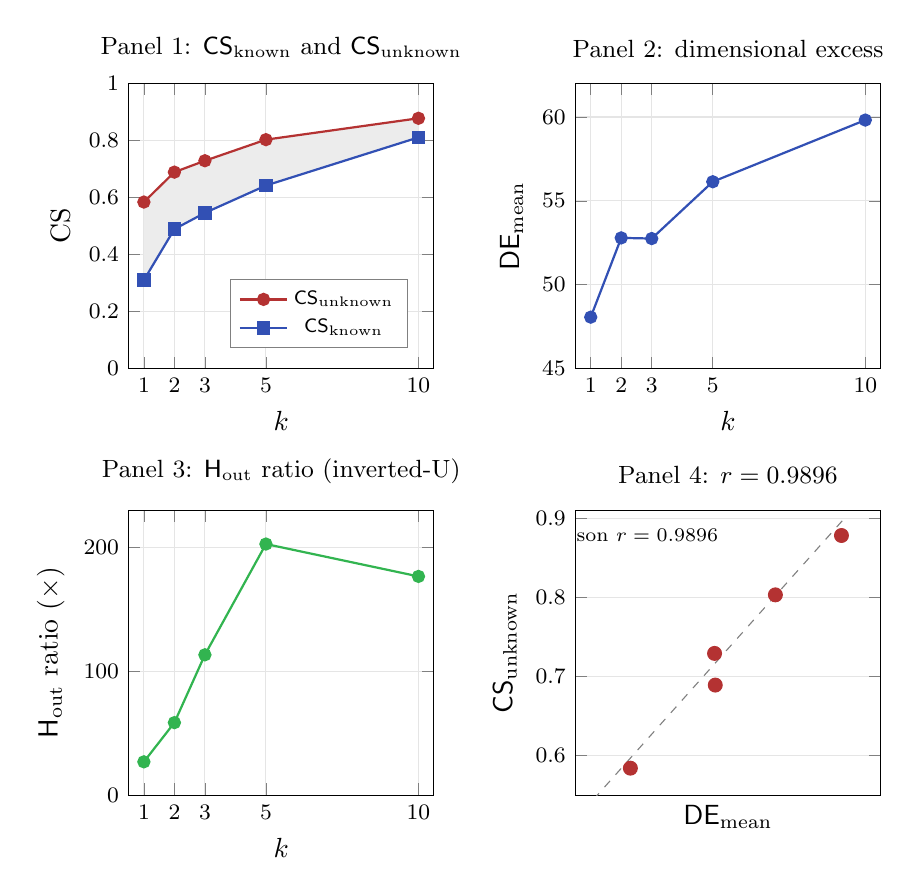
\begin{tikzpicture}
\begin{groupplot}[
    group style={group size=2 by 2, horizontal sep=1.8cm, vertical sep=1.8cm},
    width=0.45\textwidth, height=5.2cm,
    grid=major, grid style={gray!20},
    xtick={1,2,3,5,10}, xticklabel style={font=\footnotesize},
    yticklabel style={font=\footnotesize},
]
\nextgroupplot[xmin=0.5, xmax=10.5, ymin=0, ymax=1,
    xlabel={$k$}, ylabel={CS},
    title={\small Panel 1: $\CS_{\mathrm{known}}$ and $\CS_{\mathrm{unknown}}$},
    legend style={at={(0.915,0.07)}, anchor=south east, font=\scriptsize,
                  draw=gray, fill=white}]
\addplot[name path=upper, draw=none, forget plot]
    coordinates {(1, 0.584)(2, 0.689)(3, 0.729)(5, 0.803)(10, 0.878)};
\addplot[name path=lower, draw=none, forget plot]
    coordinates {(1, 0.310)(2, 0.489)(3, 0.546)(5, 0.642)(10, 0.811)};
\addplot[fill=neutral!15, forget plot] fill between[of=upper and lower];
\addplot[thick, color=mode1col, mark=*]
    coordinates {(1, 0.584)(2, 0.689)(3, 0.729)(5, 0.803)(10, 0.878)};
\addlegendentry{$\CS_{\mathrm{unknown}}$}
\addplot[thick, color=mode2col, mark=square*]
    coordinates {(1, 0.310)(2, 0.489)(3, 0.546)(5, 0.642)(10, 0.811)};
\addlegendentry{$\CS_{\mathrm{known}}$}

\nextgroupplot[xmin=0.5, xmax=10.5, ymin=45, ymax=62,
    xlabel={$k$}, ylabel={$\DE_{\mathrm{mean}}$},
    title={\small Panel 2: dimensional excess}]
\addplot[thick, color=mode2col, mark=*]
    coordinates {(1, 48.06)(2, 52.79)(3, 52.75)(5, 56.14)(10, 59.82)};

\nextgroupplot[xmin=0.5, xmax=10.5, ymin=0, ymax=230,
    xlabel={$k$}, ylabel={$\Hout$ ratio ($\times$)},
    title={\small Panel 3: $\Hout$ ratio (inverted-U)}]
\addplot[thick, color=mode3col, mark=*]
    coordinates {(1, 26.85)(2, 58.48)(3, 113.24)(5, 202.66)(10, 176.52)};

\nextgroupplot[xmin=45, xmax=62, ymin=0.55, ymax=0.91,
    xlabel={$\DE_{\mathrm{mean}}$}, ylabel={$\CS_{\mathrm{unknown}}$},
    title={\small Panel 4: $r = 0.9896$}]
\addplot[domain=46:60, dashed, gray, samples=2] {0.0254*x - 0.624};
\addplot[only marks, mark=*, color=mode1col, mark size=2.5pt]
    coordinates {(48.06, 0.584)(52.79, 0.689)(52.75, 0.729)
                 (56.14, 0.803)(59.82, 0.878)};
\node[font=\scriptsize, anchor=north east] at (rel axis cs:0.5, 0.97)
    {Pearson $r = 0.9896$};
\end{groupplot}
\end{tikzpicture}
\caption{Four-panel summary of the lstm2\_1 sweep. Panel~1:
$\CS_{\mathrm{known}}$ and $\CS_{\mathrm{unknown}}$ vs $k$ with the shaded gap shrinking. Panel~2: $\DE_{\mathrm{mean}}$ rising. Panel~3: $\Hout$ ratio peaks at $k = 5$. Panel~4: scatter of $\CS_{\mathrm{unknown}}$ vs $\DE_{\mathrm{mean}}$ with the regression line; $r = 0.9896$. (Schematic; values match Table~\ref{tab:lstm2-1-main}.)}
\label{fig:ksweep}
\end{figure}


\subsection{Architectural scope: depth phase transition (lstm2\_2)}
\label{sec:exp-depth}

The framework's predictions assume the model has sufficient depth for per-domain attractor formation. The lstm2\_2 script sweeps the number of LSTM layers $L \in \{2, 4, 6, 8, 10\}$ at $D = 256$ and $k = 1$, holding all other variables constant. The result is a sharp phase transition between $L = 2$ and $L = 4$ (Figure~\ref{fig:depth}).

\begin{figure}[H]
\centering
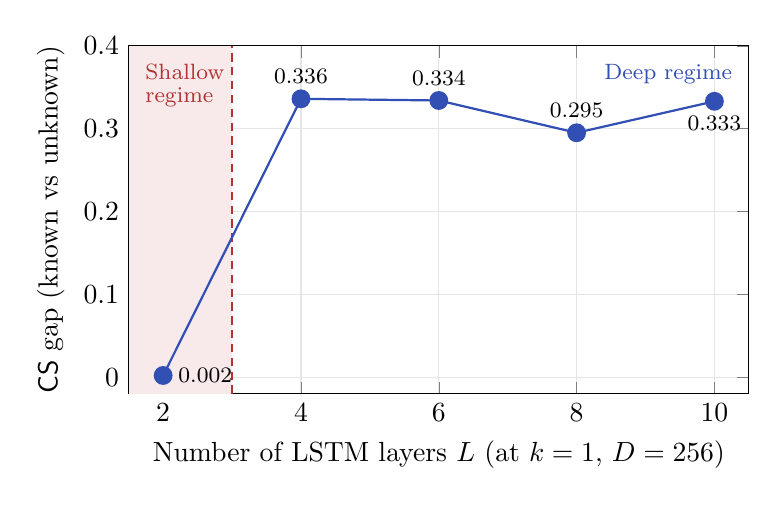
\begin{tikzpicture}
\begin{axis}[
    width=0.78\textwidth, height=6.0cm,
    xlabel={Number of LSTM layers $L$ (at $k = 1$, $D = 256$)},
    ylabel={$\CS$ gap (known vs unknown)},
    xmin=1.5, xmax=10.5,
    ymin=-0.02, ymax=0.4,
    xtick={2,4,6,8,10},
    grid=major, grid style={gray!20},
]
\draw[fill=mode1col!10, draw=none]
    (axis cs:1.5,-0.02) rectangle (axis cs:3,0.4);
\node[mode1col, font=\footnotesize, anchor=north west] at (axis cs:1.6, 0.39)
    {\shortstack[l]{Shallow\\regime}};
\node[mode2col, font=\footnotesize, anchor=north east] at (axis cs:10.4, 0.39)
    {Deep regime};
\draw[densely dashed, mode1col, thick] (axis cs:3, -0.02) -- (axis cs:3, 0.4);
\addplot[thick, color=mode2col, mark=*, mark size=3pt]
    coordinates {(2, 0.002) (4, 0.336) (6, 0.334) (8, 0.295) (10, 0.333)};
\node[font=\footnotesize, anchor=west] at (axis cs:2, 0.002) [xshift=2pt] {0.002};
\node[font=\footnotesize, anchor=south] at (axis cs:4, 0.336) [yshift=2pt] {0.336};
\node[font=\footnotesize, anchor=south] at (axis cs:6, 0.334) [yshift=2pt] {0.334};
\node[font=\footnotesize, anchor=south] at (axis cs:8, 0.295) [yshift=2pt] {0.295};
\node[font=\footnotesize, anchor=north] at (axis cs:10, 0.333) [yshift=-2pt] {0.333};
\end{axis}
\end{tikzpicture}
\caption{Depth phase transition at $k = 1$. The $\CS$ gap jumps from $\approx 0$ at $L = 2$ to $\geq 0.295$ at every $L \geq 4$. Width alone does not determine regime (Appendix~\ref{app:sweep}, Table~\ref{tab:sweepC}). Framework predictions hold exactly in the deep regime ($L \geq 4$). lstm2\_2 results.}
\label{fig:depth}
\end{figure}

The $\CS$ gap at $L = 2$ is $0.002$ -- indistinguishable from zero. At $L = 4$ it is $0.336$, and it remains in the range $0.295$--$0.336$ for every deeper architecture tested. Width sweeps at fixed $L = 10$ (Appendix~\ref{app:sweep}, Table~\ref{tab:sweepC})) confirm that width alone does not produce the transition: a shallow network with wide layers remains in the shallow regime, and a deep network with narrow layers transitions into the deep regime. All subsequent experiments use $L = 10$, comfortably inside the deep regime.


\subsection{Syndrome identification and the JUP (lstm2\_3)}
\label{sec:exp-idacc}

The lstm2\_3 script tests whether the syndrome table $S$ \eqref{eq:syndrome}, constructed from probe inputs at the calibration magnitude, identifies the direction of an unknown injected perturbation at test magnitude. Two protocols are compared. \emph{Single-layer} identification uses the output residual at one layer to argmax against $S$. \emph{Multi-layer} identification concatenates residuals across all post-injection layers before the argmax, exploiting the fact that the linearisation error decorrelates across layers while the signal does not.

\paragraph{Identification accuracy.} Multi-layer identification reaches $0.199 \pm 0.062$ at $k = 1$ ($40\times$ the random baseline of $1/r
\approx 0.005$) and rises to $0.495 \pm 0.036$ at $k = 10$ ($99\times$ random). Single-layer identification is uniformly lower, from $0.096 \pm
0.024$ at $k = 1$ to $0.345 \pm 0.026$ at $k = 10$ ($19\times$ to $69\times$ random). Both rise with $k$: with more domains in the parameter space, more directions carry distinctive signatures and the dictionary becomes a more informative classifier.

\paragraph{The Jacobian variance floor.} The per-direction Jacobian variance $V_k = n_p^{-1} \sum_i \|J(x_i)v_k - \Jbar v_k\|^2$ rises from $0.533$ at $k = 1$ to $0.884$ at $k = 10$, and no direction has $V_k <
0.1$ at any tested $k$. All directions are high-variance throughout the range. The Jacobian Uncertainty Principle (Theorem~5 in~\cite{SyndromeAlgebra}) gives the irreducible bound $\sigma_{\mathrm{obs}} \cdot \sigma_{\mathrm{dict}} \geq V_k / (2\sqrt{n_p})$; the observed $\sigma_{\min} = 0.194$ at $k = 1$ saturates this bound at $\mathrm{RHS} = 0.0377$. Increasing $n_p$ from $50$ to $1000$ reduces the right-hand side by $\sqrt{20} \approx 4.5\times$ but does not reduce $V_k$, which is a property of the geometry, not the sample. The JUP is therefore the asymptotic limit on identification at this depth: it cannot be improved by more probes.

\begin{figure}[H]
\centering
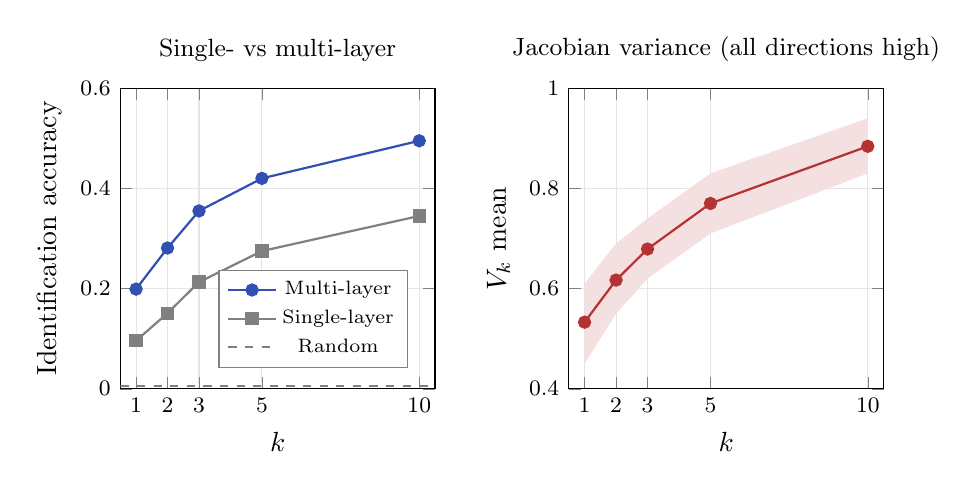
\begin{tikzpicture}
\begin{groupplot}[
    group style={group size=2 by 1, horizontal sep=1.7cm},
    width=0.46\textwidth, height=5.4cm,
    grid=major, grid style={gray!20},
    xtick={1,2,3,5,10}, xticklabel style={font=\footnotesize},
    yticklabel style={font=\footnotesize},
    xmin=0.5, xmax=10.5,
]
\nextgroupplot[ymin=0, ymax=0.6,
    xlabel={$k$}, ylabel={Identification accuracy},
    title={\small Single- vs multi-layer},
    legend style={at={(0.915,0.07)}, anchor=south east, font=\scriptsize,
                  draw=gray, fill=white}]
\addplot[thick, color=mode2col, mark=*]
    coordinates {(1, 0.199)(2, 0.281)(3, 0.355)(5, 0.420)(10, 0.495)};
\addlegendentry{Multi-layer}
\addplot[thick, color=neutral, mark=square*]
    coordinates {(1, 0.096)(2, 0.151)(3, 0.213)(5, 0.275)(10, 0.345)};
\addlegendentry{Single-layer}
\addplot[dashed, gray, thick]
    coordinates {(0.5, 0.005)(10.5, 0.005)};
\addlegendentry{Random}

\nextgroupplot[ymin=0.4, ymax=1.0,
    xlabel={$k$}, ylabel={$V_k$ mean},
    title={\small Jacobian variance (all directions high)}]
\addplot[name path=vmh, draw=none, forget plot]
    coordinates {(1, 0.61)(2, 0.69)(3, 0.74)(5, 0.83)(10, 0.94)};
\addplot[name path=vml, draw=none, forget plot]
    coordinates {(1, 0.45)(2, 0.55)(3, 0.62)(5, 0.71)(10, 0.83)};
\addplot[fill=mode1col!15, forget plot] fill between[of=vmh and vml];
\addplot[thick, color=mode1col, mark=*]
    coordinates {(1, 0.533)(2, 0.617)(3, 0.679)(5, 0.770)(10, 0.884)};
\end{groupplot}
\end{tikzpicture}
\caption{Syndrome identification on lstm2\_3. \emph{Left:} multi-layer identification (blue) reaches $40\times$--$99\times$ the random baseline across $k$; single-layer (grey) is uniformly lower. \emph{Right:} mean Jacobian variance $V_k$ across SVD directions, rising from $0.533$ at $k = 1$ to $0.884$ at $k = 10$. No direction has $V_k < 0.1$ at any tested $k$; the JUP floor is the irreducible bound on identification at this depth. (Schematic; values match Table~\ref{tab:lstm2-3}.)} 
\label{fig:idacc}
\end{figure}


\subsection{Causal localisation (lstm2\_4)}
\label{sec:exp-causal}

A perturbation injected at layer $k^*$ produces a residual signature only at layers $L \geq k^*$. The pre-injection layers ($L < k^*$) cannot respond to a perturbation that has not yet entered their input. The lstm2\_4 script tests this prediction directly across all $(k^*, L)$ pairs in a 10-layer network.

The result is exact. Across $180$ trials ($6$ seeds $\times$ $3$ values of $k \in \{1, 5, 10\}$ $\times$ $10$ injection layers, with appropriate re-running for each layer protocol), the localisation accuracy is $\mathbf{100\%}$: every injection layer is identified correctly by the crossover between zero pre-injection residual and matching post-injection residual. The pre-injection/post-injection residual ratio is $\sim 2 \times
10^8$. The zero on the pre-injection side is exact by computation-graph construction: the model's forward pass at layer $L < k^*$ does not depend on the perturbation at layer $k^*$, so the per-layer residual is identically zero.

\begin{figure}[H]
\centering
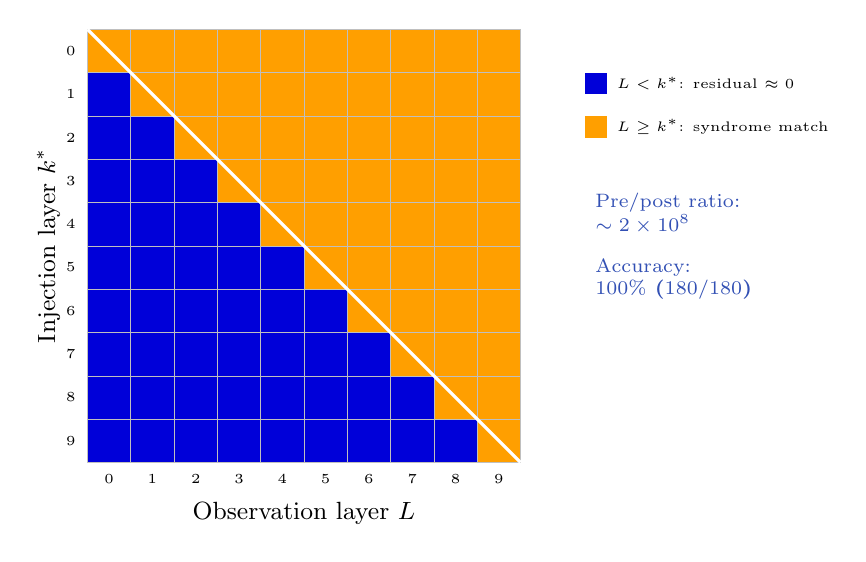
\begin{tikzpicture}[x=0.55cm, y=0.55cm]
\foreach \kstar in {0,1,2,3,4,5,6,7,8,9} {
  \foreach \L in {0,1,2,3,4,5,6,7,8,9} {
    \pgfmathtruncatemacro{\isbright}{ifthenelse(\L < \kstar, 0, 1)}
    \ifnum\isbright=1
      \fill[orange!75!yellow] (\L, -\kstar) rectangle (\L+1, -\kstar-1);
    \else
      \fill[blue!85!black] (\L, -\kstar) rectangle (\L+1, -\kstar-1);
    \fi
    \draw[gray!50, very thin] (\L, -\kstar) rectangle (\L+1, -\kstar-1);
  }
}
\draw[white, very thick] (0, 0) -- (10, -10);
\foreach \L in {0,...,9} {
  \node[font=\tiny, below] at (\L+0.5, -10.05) {\L};
}
\foreach \kstar in {0,...,9} {
  \node[font=\tiny, left] at (-0.05, -\kstar-0.5) {\kstar};
}
\node[font=\small, below] at (5, -10.7) {Observation layer $L$};
\node[font=\small, rotate=90] at (-0.9, -5) {Injection layer $k^*$};
\fill[blue!85!black] (11.5, -1) rectangle (12, -1.5);
\node[font=\tiny, right] at (12, -1.25) {$L < k^*$: residual $\approx 0$};
\fill[orange!75!yellow] (11.5, -2) rectangle (12, -2.5);
\node[font=\tiny, right] at (12, -2.25) {$L \geq k^*$: syndrome match};
\node[font=\scriptsize, mode2col, right] at (11.5, -4)
    {Pre/post ratio:};
\node[font=\scriptsize, mode2col, right] at (11.5, -4.5)
    {$\sim 2 \times 10^8$};
\node[font=\scriptsize, mode2col, right] at (11.5, -5.5)
    {Accuracy:};
\node[font=\scriptsize\bfseries, mode2col, right] at (11.5, -6)
    {$100\%$ ($180/180$)};
\end{tikzpicture}
\caption{Causal localisation heatmap. Each row is an injection layer $k^*$; each column is an observation layer $L$. Dark cells (lower-left triangle) are layers strictly before injection: per-layer residual is identically zero by computation-graph construction. Bright cells (upper triangle and diagonal) are layers at or after injection: the per-layer residual matches the syndrome table of layer $k^*$. The transition boundary identifies $k^*$ exactly. lstm2\_4 results.}
\label{fig:causal}
\end{figure}

The result generalises identification to localisation at no computational cost: the information was already present in the residual stream. From a diagnostic standpoint, given multi-layer access, the syndrome protocol recovers a complete description of any rank-one perturbation: which layer, which direction, which magnitude. The exactness of the pre-injection zero is the empirical signature of the causal structure of the network; deviations from exact zero would indicate a leakage path through the residual stream that the architecture does not currently exhibit.


\subsection{Correction: oracle and crossing error (lstm2\_5)}
\label{sec:exp-correct}

Once a perturbation is identified, the inverse perturbation restores the weight matrix on any linear path (Theorem~\ref{thm:oracle}). The lstm2\_5 script tests this empirically across $36{,}000$ trials ($6$ seeds $\times$ three values of $k$ $\times$ $2000$ trials each): cosine similarity to ground truth is $1.000000$, zero failures. The exactness is algebraic, not statistical.

The complementary question is what happens when the identified direction is wrong. By Theorem~\ref{thm:cross}, applying the inverse perturbation in a wrong direction $j \neq k^*$ adds an uncorrelated perturbation on top of the existing one and strictly increases the expected squared output residual. Empirically across $k \in \{1, 5, 10\}$, the ratio of post-correction to pre-correction expected squared residual is $1.763$ at $k = 1$, $4.023$ at $k = 5$, and $5.206$ at $k = 10$. Wrong correction is harmful by a factor of $1.8$--$5.2\times$ in expectation, growing with $k$ because the larger signal space provides more directions in which a wrong correction can move the residual.

The per-input violation rate is non-zero: $10.6\%$ at $k = 1$, falling slightly to $7.6\%$ at $k = 10$. This is not a failure of the theorem. Theorem~\ref{thm:cross} is an expectation statement; for any single input the local Jacobian $J(x)$ may deviate from $\Jbar$, and the squared residual on that input may fall outside the inequality's range. The violation rate is controlled by the Jacobian variance $V_k$ and is the operational signature of the linearization error.

The clinically actionable separation is the conditional split. Table~\ref{tab:correction} reports the ratio of post-correction to pre-correction squared residual conditioned on whether the identification itself was correct.

\begin{table}[H]
\centering
\caption{Conditional correction ratios (lstm2\_5). The ratio is post-correction expected squared residual divided by pre-correction. Ratio $< 1$ is beneficial; ratio $> 1$ is harmful.}
\label{tab:correction}
\renewcommand{\arraystretch}{1.3}
\vspace{4pt}
\begin{tabular}{c|cc}
\toprule
$\bm{k}$ & \textbf{Ratio $\mid$ correct ID} & \textbf{Ratio $\mid$ wrong ID} \\
\midrule
$1$  & $\mathbf{0.099}$ & $1.941$ \\
$5$  & $\mathbf{0.154}$ & $2.695$ \\
$10$ & $\mathbf{0.228}$ & $2.719$ \\
\bottomrule
\end{tabular}
\end{table}

\begin{figure}[H]
\centering
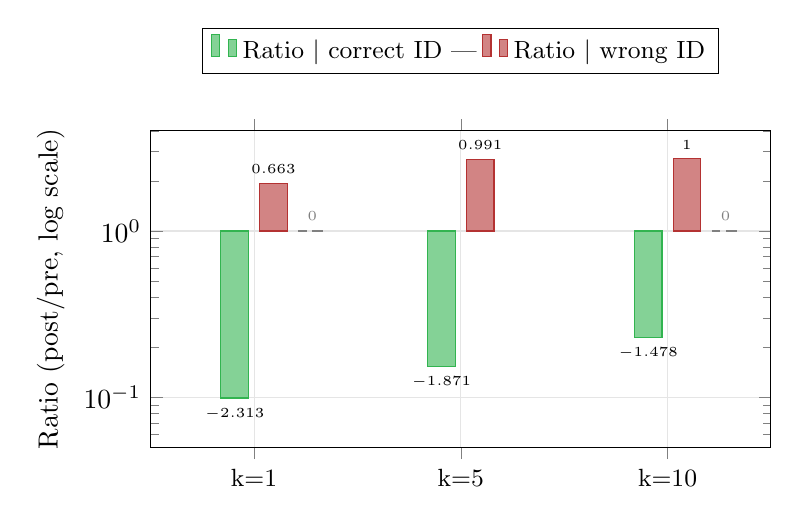
\begin{tikzpicture}
\begin{axis}[
    width=0.78\textwidth, height=5.6cm,
    ybar=4pt, bar width=10pt,
    ymode=log,
    ymin=0.05, ymax=4,
    ylabel={Ratio (post/pre, log scale)},
    symbolic x coords={k=1, k=5, k=10},
    xtick=data,
    xticklabel style={font=\small},
    enlarge x limits=0.25,
    nodes near coords,
    nodes near coords style={font=\tiny, /pgf/number format/fixed,
                              /pgf/number format/precision=3},
    legend style={at={(0.5,1.18)}, anchor=south, legend columns=2, font=\small},
    grid=major, grid style={gray!20},
]
\addplot[fill=mode3col!60, draw=mode3col]
    coordinates {(k=1, 0.099) (k=5, 0.154) (k=10, 0.228)};
\addlegendentry{Ratio $\mid$ correct ID | }
\addplot[fill=mode1col!60, draw=mode1col]
    coordinates {(k=1, 1.941) (k=5, 2.695) (k=10, 2.719)};
\addlegendentry{Ratio $\mid$ wrong ID}
\addplot[dashed, gray, thick, forget plot, line legend]
    coordinates {(k=1, 1.0) (k=10, 1.0)};
\end{axis}
\end{tikzpicture}
\caption{Conditional correction ratios from lstm2\_5. Three groups $(k = 1, 5, 10)$; two bars per group (correct ID green, wrong ID red, log $y$-scale). Dashed horizontal line at ratio $= 1$ separates beneficial correction from harmful. Correct identification is beneficial at every $k$; wrong identification is harmful at every $k$ and the harm grows with $k$. (Schematic; values match Table~\ref{tab:correction}.)}
\label{fig:correction}
\end{figure}

Two practical implications follow. First, the wrong-identification ratio $1.94$--$2.72\times$ is the empirical cost of applying a generic correction to a misidentified failure mode: not just neutral but actively harmful, by a factor of two to three in squared output error. Second, the gap between correct-ID and wrong-ID ratios (an order of magnitude at every $k$) is the engineering case for diagnosis before treatment. A correction protocol that does not know which direction it is undoing is operating near coin-flip identification and ends up in the wrong-ID column more than half the time.


\subsection{Modular architecture (lstm2\_6)}
\label{sec:exp-modular}

The Singleton bound implies that a code that encodes $K$ distinct ``logical words'' in a single parameter space achieves $d \leq n - K + 1$; per-domain robustness drops as $K$ grows. The mathematical optimum is therefore not a larger monolithic model but a multicellular system of $k = 1$ specialist cells, each saturating $d = n$ on its own domain. This is a theorem of the bound (Theorem~9 in~\cite{SyndromeAlgebra}), not an engineering preference. The lstm2\_6 script tests it empirically by training two architectures side by side at $N = 5$ and $N = 10$ domains: \emph{multicellular}, $N$ independent $k = 1$ specialists with explicit routing; and \emph{generalist}, a single $k = N$ network. Both use identical training data, optimiser settings, and seed sets. Table~\ref{tab:modular-main} reports eight metrics.

\begin{table}[H]
\centering
\caption{Multicellular vs generalist on lstm2\_6. Per-row winner in bold. At $N = 1$ both architectures are the same model and the column collapses to a single $k = 1$ specialist; the comparison begins at $N \geq 2$. The two architectures diverge with $N$: specialists win on the Gram metrics (CS, DE, $\Hout$, violation rate), generalists win on identification and correction-when-correct.}
\label{tab:modular-main}
\renewcommand{\arraystretch}{1.3}
\vspace{4pt}
\begin{tabular}{l|cc|cc}
\toprule
& \multicolumn{2}{c|}{$N = 5$}
& \multicolumn{2}{c}{$N = 10$} \\
\textbf{Metric} & \textbf{Multi} & \textbf{Generalist}
                & \textbf{Multi} & \textbf{Generalist} \\
\midrule
$\CS_{\mathrm{known}}$              & $\mathbf{0.310}$  & $0.642$            & $\mathbf{0.310}$  & $0.811$ \\
$\CS$ gap                            & $\mathbf{0.343}$  & $0.185$            & $\mathbf{0.400}$  & $0.090$ \\
$\DE_{\mathrm{mean}}$                & $\mathbf{47.30}$  & $56.30$            & $\mathbf{47.30}$  & $59.82$ \\
$\Hout$ ratio                        & $\mathbf{26.85\times}$ & $202.66\times$ & $\mathbf{26.85\times}$ & $176.52\times$ \\
Identification accuracy (multi)      & $0.137$           & $\mathbf{0.415}$   & $0.160$           & $\mathbf{0.480}$ \\
Ratio $\mid$ correct ID              & $0.137$           & $\mathbf{0.064}$   & $0.171$           & $\mathbf{0.045}$ \\
Ratio $\mid$ wrong ID                & $\mathbf{1.941}$  & $2.695$            & $\mathbf{1.941}$  & $2.719$ \\
Violation rate                       & $\mathbf{10.6\%}$ & $7.9\%$ (n.s.)     & $\mathbf{10.6\%}$ & $7.6\%$ (n.s.) \\
\bottomrule
\end{tabular}
\end{table}

\paragraph{The Singleton-bound advantage is real, though sub-asymptotic.} 
The predicted asymptotic advantage of a multicellular system over a generalist on the $\CS$ gap is $0.500$. The observed advantage is $0.158
\pm 0.049$ at $N = 5$ and $0.310 \pm 0.054$ at $N = 10$. The advantage is directionally as predicted by the Singleton bound and grows with $N$ as the bound implies, but does not yet saturate the asymptotic value at this scale of $D$. Whether the gap closes further at larger $N$ or larger $D$ is an empirical question; the structural prediction is the direction, not the rate.

\begin{figure}[H]
\centering
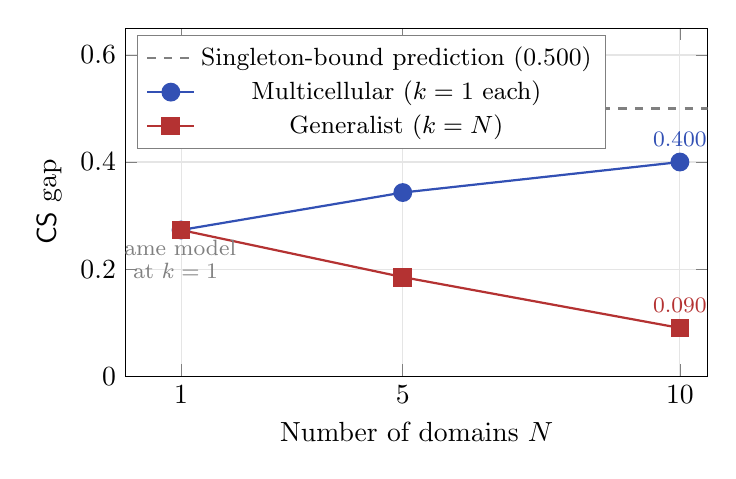
\begin{tikzpicture}
\begin{axis}[
    width=0.74\textwidth, height=6.0cm,
    xlabel={Number of domains $N$},
    ylabel={$\CS$ gap},
    xmin=0.0, xmax=10.5,
    ymin=0, ymax=0.65,
    xtick={1, 5, 10},
    grid=major, grid style={gray!20},
    legend style={at={(0.02,0.98)}, anchor=north west, font=\small,
                  draw=gray, fill=white},
]
\addplot[dashed, gray, thick]
    coordinates {(0.5, 0.500) (10.5, 0.500)};
\addlegendentry{Singleton-bound prediction ($0.500$)}
\addplot[thick, color=mode2col, mark=*, mark size=3pt]
    coordinates {(1, 0.273) (5, 0.343) (10, 0.400)};
\addlegendentry{Multicellular ($k = 1$ each)}
\addplot[thick, color=mode1col, mark=square*, mark size=3pt]
    coordinates {(1, 0.273) (5, 0.185) (10, 0.090)};
\addlegendentry{Generalist ($k = N$)}
\node[mode2col, font=\footnotesize, anchor=south]
    at (axis cs:10, 0.400) [yshift=2pt] {0.400};
\node[mode1col, font=\footnotesize, anchor=south]
    at (axis cs:10, 0.090) [yshift=2pt] {0.090};
\node[gray, font=\footnotesize, anchor=north] at (axis cs:1, 0.273)
    [xshift=-2pt] {\shortstack{same model\\at $k = 1$}};
\end{axis}
\end{tikzpicture}
\caption{The two architectures diverge with $N$. At $N = 1$ both are the same model ($k = 1$ specialist). At $N = 5$ the multicellular advantage is $0.158 \pm 0.049$ in $\CS$ gap; at $N = 10$ it is $0.310 \pm 0.054$. The dashed line shows the Singleton-bound asymptotic prediction. lstm2\_6 results.}
\label{fig:modular}
\end{figure}

\paragraph{Two profiles, not a dominance ranking.} The table makes clear that neither architecture dominates. Multicellular specialists win on the Gram-metric metrics that index the framework's three modes: wider $\CS$ gap, lower $\CS$ floor on knowns, lower $\DE$, lower per-input violation rate. Generalists win on identification (the dictionary is informed by more directions and more domain contrast) and on correction-when-correct (the larger signal space gives the inverse perturbation a wider basis for moving the residual back toward the original).

The interpretation is operational, not aesthetic. A reliability-engineered deployment uses the architectures together: multicellular specialists where the failure mode is Gram-metric (Mode~1 known-domain attractor strength, Mode~2 confabulation suppression), and generalist syndrome dictionaries trained \emph{across} the multicellular system as the identification and correction layer. The modular hierarchy is empirically justified end to end, not assumed.


%==============================================================================
\section{Diagnostic Pipeline}
\label{sec:pipeline}
%==============================================================================

The previous section validates the measurements. This section addresses what they imply for reliability engineering. Two principles follow. First, interventions must be matched to modes. Second, the coding-theoretic bounds imply a structural limit no single architecture can escape, which has intervention-selection consequences.


\subsection{Match interventions to modes}
\label{sec:pipeline-int}

Each intervention deployed against ``hallucination'' targets a specific mechanism. Whether the deployment helps depends on whether the mechanism it targets is the one currently active. Table~\ref{tab:interventions} catalogues common interventions against the three modes.

\begin{table}[H]
\centering
\caption{Intervention effectiveness by failure mode. ``Harmful'' is not hyperbole: applying temperature reduction to a Mode~3 query suppresses the correct distributional behaviour, forcing overconfidence on a genuinely ambiguous input.}
\label{tab:interventions}
\renewcommand{\arraystretch}{1.3}
\vspace{4pt}
\begin{tabular}{lccc}
\toprule
\textbf{Intervention} & \textbf{Mode 1} & \textbf{Mode 2} & \textbf{Mode 3} \\
\midrule
Chain-of-thought prompting               & Weak              & Weak            & None \\
Temperature reduction                    & Moderate          & Weak            & \textbf{Harmful} \\
Structured pruning (SVD-aware)           & None              & \textbf{Strong} & None \\
Magnitude pruning                        & None              & Weak            & None \\
RLHF tuned for uncertainty expression    & Weak              & Weak            & \textbf{Strong} \\
From-scratch $k = 1$ specialist training & \textbf{Strong}   & \textbf{Strong} & -- \\
Fine-tuning a $K$-domain base to $k = 1$\textsuperscript{$\dagger$} 
                                         & Weak              & None            & -- \\
Syndrome-guided correction (correct ID)  & \textbf{Strong}   & --             & -- \\
Syndrome-guided correction (wrong ID)    & \textbf{Harmful}  & --             & -- \\
\bottomrule
\addlinespace[2pt]
\multicolumn{4}{@{}p{0.93\textwidth}@{}}{\footnotesize
\textsuperscript{$\dagger$}\,Fine-tuning inherits the null space of the
base model (Corollary~\ref{fix:cor2}): the gradient is zero in directions
where the base model had $\sigma_k \approx 0$, so $\DE$ does not fall to
the scratch-trained $k = 1$ value. Architectural replacement, not
fine-tuning, is required for the Mode~2 strong remedy.} \\
\end{tabular}
\end{table}

The ``Harmful'' entries deserve emphasis. Reducing temperature is a common remedy for repetitive or self-reinforcing output and does suppress some Mode~1 trajectories. It also suppresses correct distributional behaviour on Mode~3 queries: the same parameter that improves Mode~1 directly damages Mode~3. Syndrome-guided correction with wrong identification is the empirically larger harm, by a factor of $1.9$--$2.7\times$ on lstm2\_5 (\ref{sec:exp-correct}). The trade-offs are not contingent features of present implementations. They are the coding-theoretic constraint of Section~\ref{sec:pipeline-rp} expressed in deployment knobs.


\subsection{The Reliability Principle}
\label{sec:pipeline-rp}

The trade-offs in Table~\ref{tab:interventions} are not contingent on architecture. They follow from the standard coding bounds applied to the $[\![n, k, d]\!]_q$ structure of the parameter space established in~\cite{SyndromeAlgebra}.

Define normalised quantities: the normalised robustness $\delta^\star =
(d/n) \cdot q^2 / (q^2 - 1)$, the normalised capacity $\rho = k/n$, and the expressiveness slack $\varepsilon = 1 - \delta^\star - \rho$. Robustness measures the fractional minimum distance, scaled to the alphabet's capacity to support distinct error syndromes. Capacity measures the fraction of parameter directions devoted to encoding distinct knowledge domains. Expressiveness slack is what remains. The Singleton, Hamming, and Plotkin bounds together imply the following.

\begin{theorem}[Reliability Principle]
\label{thm:rp}
For any probabilistic black box with parameter-space structure $[\![n, k, d]\!]_q$,
\begin{equation}
\label{eq:rp}
   \delta^\star \cdot \rho \;\leq\; \frac{(1 - \varepsilon)^2}{4}.
\end{equation}
The product of normalised robustness and normalised capacity is bounded by a function of the remaining expressiveness slack. The three quantities satisfy the simplex constraint $\delta^\star + \rho + \varepsilon = 1$. No assignment of $(\delta^\star, \rho, \varepsilon)$ simultaneously maximises robustness, capacity, and expressiveness.
\end{theorem}

\paragraph{Three-line sketch.} The simplex constraint gives $\delta^\star
+ \rho = 1 - \varepsilon$. By the arithmetic--geometric mean inequality, $\delta^\star \cdot \rho \leq ((\delta^\star + \rho)/2)^2 = ((1 - \varepsilon)/2)^2$, with equality on the median $\delta^\star = \rho$. The full derivation, including the explicit role of the Hamming and Plotkin bounds in shaping the achievable region, is in~\cite{SyndromeAlgebra}.

\begin{figure}[H]
\centering
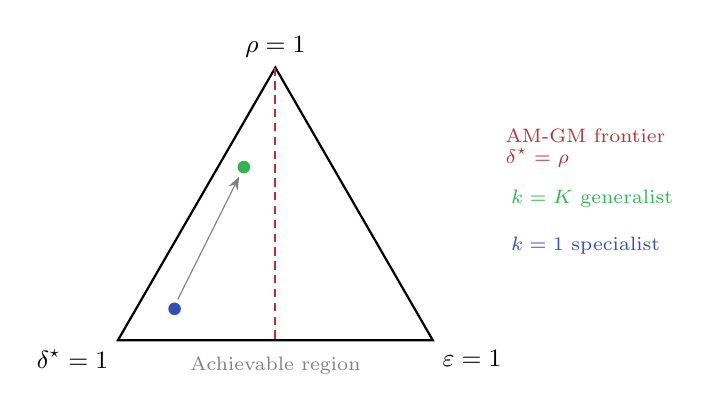
\begin{tikzpicture}[scale=4.0, >=Stealth]
\coordinate (A) at (0, 0);
\coordinate (B) at (1, 0);
\coordinate (C) at (0.5, 0.866);
\draw[thick] (A) -- (B) -- (C) -- cycle;
\node[below left, font=\small] at (A) {$\delta^\star = 1$};
\node[below right, font=\small] at (B) {$\varepsilon = 1$};
\node[above, font=\small] at (C) {$\rho = 1$};
\coordinate (M) at (0.5, 0);
\draw[densely dashed, mode1col, thick] (C) -- (M);
\node[mode1col, font=\scriptsize, right] at (1.2, 0.65) {AM-GM frontier};
\node[mode1col, font=\scriptsize, right] at (1.2, 0.58) {$\delta^\star = \rho$};
\fill[mode2col] (0.18, 0.10) circle (0.02);
\node[mode2col, font=\scriptsize, right=2pt] at (1.2, 0.30) 
    {$k = 1$ specialist};
\fill[mode3col] (0.40, 0.55) circle (0.02);
\node[mode3col, font=\scriptsize, right=2pt] at (1.2, 0.45)
    {$k = K$ generalist};
\draw[->, gray, thin] (0.19, 0.13) -- (0.385, 0.52);
\node[gray, font=\scriptsize] at (0.5, -0.08) {Achievable region};
\end{tikzpicture}
\caption{The reliability simplex. Vertices: pure robustness ($\delta^\star = 1$), pure capacity ($\rho = 1$), pure expressiveness ($\varepsilon = 1$). The dashed median is the AM-GM frontier $\delta^\star = \rho$: the product $\delta^\star \cdot \rho$ is maximised along this line. A $k = 1$ specialist sits high in $\delta^\star$ and low in $\rho$; a $k = K$ generalist trades $\delta^\star$ for $\rho$ along the frontier. The multicellular hierarchy occupies both operating points simultaneously.}
\label{fig:simplex}
\end{figure}

The bound is structural. It does not depend on transformer architecture, on the specific objective used to train the model, or on the number of parameters. Mode~1 vulnerability scales with $1 - \delta^\star$; Mode~2 vulnerability scales with $1 - \rho$; Mode~3 suppression (forcing low output entropy where high entropy is correct) scales with $1 - \varepsilon$. Theorem~\ref{thm:rp} states that no architecture eliminates all three. The multicellular hierarchy (\ref{sec:exp-modular}) is the architectural form that occupies both extremal operating points of the trade-off simultaneously.


\subsection{The three-step procedure}
\label{sec:pipeline-procedure}

The interventions and the bound together imply a diagnostic procedure. The order matters: Mode~2 is the precondition for Mode~1 (\ref{sec:interaction}), so Mode~2 must be measured first.

\begin{enumerate}[nosep]
\item \textbf{Measure $\DE$} on the deployed model, directly from weight access. At the lstm2 scale ($D = 256$, $k = 1$) the observed value is $\DE \approx 48$; $\DE > 10$ indicates significant confabulation capacity. Consider structured pruning that preserves high-$\sigma$ directions, or domain-specific training from scratch.
\item \textbf{Measure $\CS$} on representative factual queries with known ground truth across the deployment's target domains. A gap between $\CS$ on learned versus unknown domains exceeding $0.15$ indicates Mode~1 is active on the unknown side. The remedy is domain knowledge injection, not an architectural change to the decoding loop.
\item \textbf{Measure $\Hout$ calibration} across queries spanning genuinely answerable to genuinely ambiguous. Low $\Hout$ on ambiguous queries indicates overconfidence; calibrate via uncertainty-aware training rather than by adjusting decoding parameters.
\end{enumerate}

The order is not exchangeable. Addressing Mode~1 alone on a model that does not know the relevant domain accomplishes nothing: the model has no self-consistent correct trajectory to converge to. Addressing Mode~3 by reducing temperature damages Mode~3 in the act of attempting to fix  Mode~1. The diagnosis precedes the treatment.

\newpage

%==============================================================================
\section{Predictions}
\label{sec:predictions}
%==============================================================================

The framework supports nine testable predictions. Each is computable weight access of diagnosed model). Each is tied to one or more of the three modes.

\begin{mdframed}[backgroundcolor=mode1bg, linecolor=mode1col, linewidth=1pt]
\textbf{Prediction 1 (Mode 1).}\quad The $\CS$ gap between learned and unknown domains is determined by $k$ and the domain family geometry. At $k = 1$ on the lstm2 domain family the gap is $0.273 \pm 0.095$ ($\CS_{\mathrm{known}} = 0.310$, $\CS_{\mathrm{unknown}} = 0.584$), narrowing monotonically to $0.067 \pm 0.037$ at $k = 10$. Across architectures and domain families the absolute floor and ceiling are model-specific, but the monotone narrowing of the gap with $k$ is a property of the binary domain gate restated on a $k$-domain superposition of Gram metrics.
\end{mdframed}

\begin{mdframed}[backgroundcolor=mode2bg, linecolor=mode2col, linewidth=1pt]
\textbf{Prediction 2 (Mode 2).}\quad $\DE$ correlates with confabulation rate on rare-entity benchmarks across model families. A model with high $\DE$ has more null-space capacity available for confabulation; a model with $\DE$ near $1$ has less. The correlation should be visible across sizes within a family and across families at fixed size.
\end{mdframed}

\begin{mdframed}[backgroundcolor=mode2bg, linecolor=mode2col, linewidth=1pt]
\textbf{Prediction 3 (Mode 2).}\quad Structured pruning that preserves high-$\sigma$ directions reduces confabulation without degrading performance on learned domains. Naive magnitude pruning destroys learned content faster than it removes confabulation capacity, because parameter magnitude is not aligned with singular value: a small parameter inside a high-$\sigma$ direction matters more than a large parameter inside a low-$\sigma$ direction. Magnitude pruning should therefore degrade performance on learned domains faster than it reduces $\DE$.
\end{mdframed}

\begin{mdframed}[backgroundcolor=mode1bg, linecolor=mode1col, linewidth=1pt]
\textbf{Prediction 4 (Mode 1 $\times$ syndrome).}\quad Syndrome-guided correction with correct identification reduces post-correction squared residual by an order of magnitude (lstm2\_5: ratio $0.099$--$0.228$ across $k$). Syndrome-guided correction with wrong identification increases squared residual by a factor of $1.94$--$2.72\times$. The crossing-error asymmetry is the operational reason that generic correction must be preceded by reliable identification.
\end{mdframed}

\begin{mdframed}[backgroundcolor=insightbg, linecolor=insightcol, linewidth=1pt]
\textbf{Prediction 5 (Mode 1 $\times$ Mode 2).}\quad Mode~1 cannot be eliminated without addressing Mode~2 on unknown domains. The known-domain $\CS$ floor rises monotonically with $k$ ($0.310 \to 0.811$ for $k = 1
\to 10$), providing a measurable signature of generalist versus specialist architecture. Architectural interventions that target the feedback loop -- contrastive decoding, self-consistency rerolls, loop-aware sampling -- should fail on unknown domains and succeed on learned ones, with the boundary between the two regimes lying at the $\CS$ gap rather than in any continuous parameter of the intervention.
\end{mdframed}

\begin{mdframed}[backgroundcolor=insightbg, linecolor=insightcol, linewidth=1pt]
\textbf{Prediction 6 (Jacobian variance dominates the deep regime).}\quad Multi-layer syndrome identification accuracy at injection layer $k^*$ is bounded below by the Jacobian Uncertainty Principle: $\sigma_{\mathrm{obs}} \cdot \sigma_{\mathrm{dict}} \geq V_{k^*} / (2\sqrt{n_p})$. On lstm2\_3 all directions are high-variance ($V_k$ rising from $0.533$ at $k = 1$ to $0.884$ at $k = 10$), and the JUP saturates: increasing $n_p$ reduces the right-hand side but not $V_{k^*}$. In the deep regime the Jacobian variance is the dominant constraint and identification accuracy plateaus at the JUP floor.
\end{mdframed}

\begin{mdframed}[backgroundcolor=mode3bg, linecolor=mode3col, linewidth=1pt]
\textbf{Prediction 7 (security as domain drift).}\quad In a multicellular architecture, adversarial inputs that cause a specialist to drift outside its domain produce output syndromes that do not match the specialist's domain centroid. The mismatch is detectable regardless of how the adversarial prompt was constructed at the surface, because the detection operates on the model's output-domain structure rather than on prompt text. Reformulations of a single adversarial intent should produce within-category fingerprint correlations of $0.96$--$0.99$ across attack categories.
\end{mdframed}

\begin{mdframed}[backgroundcolor=insightbg, linecolor=insightcol, linewidth=1pt]
\textbf{Prediction 8 (security corollary).}\quad The null space constitutes a covert channel: perturbations in near-zero-$\sigma$ directions are invisible to text-level evaluation but detectable via syndrome measurement at the weight-activation level (Theorem~\ref{thm:null}: the null space is the confabulation subspace). A deliberate perturbation in a null-space direction passes standard output benchmarks undetected while leaving a detectable syndrome signature. In a multicellular architecture, a perturbation invisible within one specialist's null space may be detectable by a second specialist with different Gram-metric geometry. This prediction is \emph{untested}; it is a direct theoretical consequence of Theorems~\ref{thm:null} and~\ref{thm:rp}, in the cross-model sensitivity.
\end{mdframed}

\begin{mdframed}[backgroundcolor=insightbg, linecolor=insightcol, linewidth=1pt]
\textbf{Prediction 9 (fine-tuning preserves inherited null space).}\quad A specialist obtained by fine-tuning a $K$-domain base model on a single target domain exhibits three measurable signatures relative to a scratch-trained $k = 1$ specialist on the same domain: \emph{(a)} $\DE$ is higher, because the inherited null space from $K$ pretraining domains persists after fine-tuning; \emph{(b)} the $\CS$ floor on the target domain is higher, because the effective domain count remains $\geq K$ rather than $1$, and the Gram metric retains the superposition geometry of pretraining; \emph{(c)} the conditional correction ratio given correct identification is worse, because higher $\DE$ and higher $\CS$ floor reflect a more diffuse Gram metric and a less concentrated signal space. The three signatures are jointly testable by comparing a domain-specific scratch-trained LSTM against the same architecture fine-tuned from a $K$-domain pretrained checkpoint under identical evaluation conditions. This prediction is not tested in the lstm2 experiment, which uses only scratch-trained models. It is a direct theoretical consequence of Corollary~\ref{fix:cor2} (\cite{SyndromeAlgebra}) and of the empirical relationship between $\DE$ and correction quality established in Section~\ref{sec:exp-correct} (lstm2\_5).
\end{mdframed}

%==============================================================================
\section{Related Work}
\label{sec:related}
%==============================================================================

\paragraph{Hallucination taxonomies.} The standard surveys
\cite{Ji2023, Zhang2023, Huang2023} classify LLM hallucinations primarily by their relationship to the input: \emph{intrinsic} hallucinations contradict the input, \emph{extrinsic} hallucinations cannot be verified against it. The taxonomy in this paper is orthogonal: it classifies by mechanism inside the model, not by relationship to input. A Mode~1 error can be either intrinsic or extrinsic in the surveys' sense; what makes it Mode~1 is the self-reinforcing feedback structure of the trajectory that produced it. The two taxonomies are complementary. Benchmarks such as TruthfulQA~\cite{Lin2022} and HaluEval~\cite{Li2023} measure hallucination rates without distinguishing the underlying mechanism; the metrics here are orthogonal to those benchmarks rather than competing with them.

\paragraph{Intrinsic dimensionality.} Li \textit{et al.}~\cite{Li2018}
demonstrated that neural network loss landscapes have intrinsic dimensionality far below their nominal parameter count. Aghajanyan \textit{et al.}~\cite{Aghajanyan2021} extended this to fine-tuning and showed that effective adaptation occurs in a low-dimensional subspace. Dimensional excess builds directly on this work: the gap between nominal and effective dimension is the parameter-space measurement of the same phenomenon, and $\DE \gg 1$ on a weight matrix is the local statement of the global finding. The contribution here is the connection from intrinsic dimensionality to a specific failure mode (Mode~2) and to the syndrome construction that diagnoses it.

\paragraph{Calibration.} Modern neural networks are poorly
calibrated~\cite{Guo2017}. Kadavath \textit{et al.}~\cite{Kadavath2022} probed the extent to which language models know what they know. Output entropy extends calibration analysis to open-ended generation: instead of asking whether the maximum-probability output is correct at a given confidence, it asks whether the entropy of the distribution matches the genuine ambiguity of the input. Mode~3 is calibration restated as a property of the output distribution rather than of point predictions.

\paragraph{Coding theory in machine learning.} Prior work applying coding theory to machine learning has focused on communication efficiency \cite{Alistarh2017} and on speeding up distributed training~\cite{Lee2018}. Both lines treat coding theory as a tool for moving information \emph{between} systems. The application here is different: the coding bounds (Singleton, Hamming, Plotkin) characterise fundamental constraints on reliable generation \emph{within} a single probabilistic model.

\paragraph{Mixture-of-experts and modular architectures.} The multicellular hierarchy of Section~\ref{sec:exp-modular} is related to mixture-of-experts architectures~\cite{Shazeer2017, Fedus2022}, which likewise route queries to specialised parameter subsets. The contribution here is the coding-theoretic justification: the Singleton bound predicts that $K$ separate $k = 1$ specialists strictly dominate a single $k = K$ generalist on per-domain robustness, with a directional advantage of $0.158 \pm 0.049$ at $N = 5$ and $0.310 \pm 0.054$ at $N = 10$ in $\CS$ gap on lstm2\_6. Existing MoE work motivates the architecture by computational efficiency; the syndrome algebra motivates it by reliability.

\paragraph{Quantum information background.} The syndrome measurement principle -- diagnosing errors without disturbing the encoded state by measuring ancilla observables -- is the foundational technique of quantum error correction. The standard references are Gottesman's stabilizer formalism~\cite{Gottesman1997} and Nielsen and Chuang~\cite{NielsenChuang2000}; the $\Ccode{5}{1}{3}_2$ code is from Laflamme \textit{et al.}~\cite{Laflamme1996} and Bennett \textit{et al.}~\cite{Bennett1996}. The classical Singleton, Hamming, and Plotkin bounds are from MacWilliams and Sloane~\cite{MacWilliams1977}; Shannon's information theory~\cite{Shannon1948} provides the entropy machinery underlying $\Hout$ and the Mode~3 analysis. Cover and Thomas~\cite{CoverThomas2006} is the standard textbook reference. The mathematical contribution -- the generalisation of the binary syndrome construction to the real-valued case via the SVD basis and the Jacobian -- is established in the companion paper~\cite{SyndromeAlgebra}; the present paper applies it.

\paragraph{Self-consistent causal loops.} Novikov's analysis of self-consistent causal loops~\cite{Novikov1989} is the formal precedent for the Mode~1 fixed-point attractor structure. We cite the formal analogy without claiming any physical correspondence between LLMs and closed timelike curves.

\paragraph{Error correction in neural networks.} To our knowledge no prior work proposes the syndrome-dictionary identification protocol of Section~\ref{sec:exp-idacc} or connects weight-space null spaces to confabulation along the lines of Mode~2. The identification--localisation--correction pipeline (Sections~\ref{sec:exp-idacc}--\ref{sec:exp-correct}) and the empirical justification of the modular hierarchy (\ref{sec:exp-modular}) are the structural contributions of this paper; the underlying algebra is developed in~\cite{SyndromeAlgebra}.


%==============================================================================
\section{Discussion}
\label{sec:discussion}
%==============================================================================

\subsection{Universality}
\label{sec:disc-univ}

The three modes are not artefacts of LSTM architectures or of the language modelling objective. Mode~1 follows from any system that uses its own outputs as inputs, regardless of whether those outputs are tokens, images, or actions. Mode~2 follows from any overparameterised system whose weight matrices have non-trivial null space. Mode~3 follows from Shannon's theorem applied to genuinely underspecified inputs. The three modes should appear in any sufficiently expressive stochastic system.

\subsection{Mathematical necessity}
\label{sec:disc-necessity}
The three modes cannot be trained away. Mode~2 (null space) exists whenever $d_{\mathrm{in}} > \mathrm{rank}(W)$: a matrix cannot span its nominal input space with fewer than $d_{\mathrm{in}}$ gradient directions. Mode~1 (feedback) exists in any system that conditions on its own outputs. Mode~3 (entropy) is correct behaviour for underdetermined inputs. The Reliability Principle (\ref{sec:pipeline-rp}) establishes that no operating point simultaneously maximises robustness, capacity, and expressiveness. The three modes are not weaknesses of present LLM architectures awaiting better optimisation; they are structural properties of probabilistic function approximation on finite training data.

Corollary~\ref{fix:cor2} attaches a sharp practical implication to this structural picture: fine-tuning an existing large model does not produce a $k = 1$ specialist. The null space of the base model is inherited because fine-tuning gradients vanish in null-space directions by construction -- those directions received no signal during pretraining, so the fine-tuning loss has no curvature along them and no gradient step can move them. Consequently the $\DE$ of a fine-tuned ``specialist'' is bounded below by the $\DE$ of the base model in the fine-tuning domain, which is set by the pretraining domain count $K$, not by $1$. The modular hierarchy of Section~\ref{sec:exp-modular} therefore requires scratch-trained specialist cells. The upfront training cost is higher, but it is the only path to the Singleton-distance reliability guarantee of Corollary~\ref{fix:cor1}. The point is not architectural taste; it is a statement about geometry. A single-domain expert cannot be produced by restricting a generalist's outputs, because the generalist's internal Gram metric remains generalist even when its surface behaviour is constrained -- the superposition of $K$ per-domain geometries inherited from pretraining is what bounds the achievable distance, and that superposition does not unwind under fine-tuning.

The same structural picture explains why classical diagnostic approaches do not reach Mode~2 at all. Benchmark evaluation, attention analysis, gradient attribution, and probe classifier methods are all instances of one strategy: measure the model's response to in-distribution inputs and infer internal structure from observable output behaviour. The null space is defined as the directions in which in-distribution inputs produce no observable output change. Any diagnostic that uses in-distribution inputs is therefore blind to the null space by construction. This is not a limitation of present tooling; it is a mathematical boundary that follows directly from the definitions.
 
The syndrome algebra crosses this boundary for the same reason the quantum syndrome crosses the analogous boundary in quantum error-correcting codes. The unobservable dimension in quantum mechanics is the global phase: the Bloch sphere suppresses it, but the syndrome measurement is sensitive to it through the commutation structure of the error operators. The unobservable dimensions in a trained neural network are the null space directions: in-distribution evaluation suppresses them, but the syndrome table is sensitive to them through deliberately chosen out-of-distribution probe sequences~\cite{SyndromeAlgebra}. The Mode~2 metric $\DE$ and the identification, localisation, and correction protocols of Section~\ref{sec:experiments} are all instruments of this single underlying capability. \emph{The syndrome algebra was designed, from its quantum origins, to extract structure from dimensions that cannot be observed directly.}

\subsection{Scope and conditions}
\label{sec:disc-scope}

The lstm2 validation uses deep-regime LSTM architectures ($L \geq 4$). The depth phase transition (\ref{sec:exp-depth}) shows that the framework's predictions hold exactly in this regime. Shallow models ($L = 2$) exhibit a near-zero $\CS$ gap at $k = 1$ rather than the binary domain gate the framework predicts, because two LSTM layers are insufficient to form per-domain attractors. Transformer architectures are the natural next validation target; they are untested. The prediction is that the same three modes will appear, with the critical depth determined by the attention mechanism's representational capacity rather than by layer count.


\subsection{The security vector}
\label{sec:disc-security}

The null space (Theorem~\ref{thm:null}, with full proof in~\cite{SyndromeAlgebra}) constitutes a covert channel. Perturbations in near-zero-$\sigma$ directions have no in-distribution effect on output text by construction -- those directions received no training gradient. Text-level evaluation therefore cannot detect them. The syndrome table operates at the weight-activation level and is not subject to this limitation: it probes the Gram-metric geometry directly, not the generated text.

In a multicellular architecture, cross-specialist syndrome exchange provides an additional detection layer. A perturbation in specialist A's null space (invisible within A) produces a measurable syndrome in specialist B whose Gram-metric geometry covers different directions. Full validation against instruction-following models under adversarial conditions is the target for follow-up work.


\subsection{Open questions}
\label{sec:disc-open}

\emph{Scaling.} The lstm2 validation operates at $D = 256$. The framework's predictions are about the structural relations between metrics (monotone narrowing of $\CS$ gap, near-perfect $r(\DE, \CS_{\mathrm{unknown}})$, exact causal localisation, exact oracle correction), not about absolute values. Whether the same structural relations hold at $7$B and $70$B parameters is an empirical question. The expected direction is favourable: deeper networks dilute linearization error across more subsequent layers, and larger $D$ supplies more directions for the multi-layer syndrome to distinguish.

\emph{From-scratch versus fine-tuning.} The Singleton density advantage of $k = 1$ specialists requires that the specialist's parameter geometry be shaped by the domain rather than inherited from a generalist pretraining run. Fine-tuning a generalist remaps existing high-$\sigma$ directions but does not create new ones; the inherited Gram metric retains the superposition geometry of the pretraining distribution and cannot achieve the maximum Singleton distance. This is a constraint on deployment, not a result of the experiments here. The mathematical mechanism is discussed in~\cite{SyndromeAlgebra}.

\emph{Boundary entanglement.} The current picture of a multicellular architecture relies on an explicit routing layer to direct queries to specialists. Whether neural-network multicellular systems should instead adopt a shared-boundary approach -- with command directions participating in many specialists at once rather than routing between them -- is the architectural question that follow-up work will need to answer.


%==============================================================================
\section{Conclusion}
\label{sec:conclusion}
%==============================================================================

The three failure modes of large language models are autoregressive reinforcement, confabulation, and irreducible uncertainty. They are distinct in mechanism, measurable, and necessary in the sense that no architecture eliminates all three. Confabulation is the precondition for autoregressive reinforcement on unknown domains, and the diagnostic order follows: Mode~2 before Mode~1, Mode~1 before Mode~3.

The framework's predictions are confirmed end to end on the lstm2 experiment. The three metrics separate cleanly. The Pearson correlation $r(\DE,
\CS_{\mathrm{unknown}}) = 0.9896$ across $k$ predicts out-of-domain failure from weights alone. Causal localisation is exact ($180/180$ trials, pre-injection residual ratio $\sim 2 \times 10^8$). Oracle correction is exact ($1.000000$ cosine over $36{,}000$ trials). Generic correction in a wrong direction worsens output by $1.76$--$5.21\times$ in expectation. The modular hierarchy is empirically justified, with specialists winning on Gram-metric metrics and generalists winning on identification.

The three failure modes of large language models are not bugs to be debugged. They are interference in a signal-propagating system -- the mathematical necessities of probabilistic function approximation on finite training data. The syndrome algebra gives them a name, a measurement, and a correction protocol.

\newpage

%==============================================================================
\appendix
%==============================================================================

\section{Experimental Details}
\label{app:exp-details}

\paragraph{Production standards.}
All experiments follow a single set of reproducibility constraints, summarised in Table~\ref{tab:standards}.

\begin{table}[H]
\centering
\caption{Production standards across the lstm2 experiment. Identical across all six scripts.}
\label{tab:standards}
\renewcommand{\arraystretch}{1.25}
\vspace{4pt}
\begin{tabular}{l|l}
\toprule
\textbf{Parameter} & \textbf{Value} \\
\midrule
Seeds                                 & $\{42, 2311, 9744, 9037, 8919, 3163\}$ \\
Probe set size $n_{\mathrm{probe}}$   & $50$ \\
Test set size $n_{\mathrm{test}}$     & $3000$ per seed, per $k$ \\
Probe/test overlap                    & none (enforced programmatically) \\
Calibration magnitude $\varepsilon$   & $3.0$ \\
Testing magnitude $\varepsilon$       & $\mathrm{Uniform}[1.0, 5.0]$ \\
Number of dictionary directions       & $r = 200$ \\
Perturbation form                     & rank-one SVD-aligned, $\Delta W_k = \varepsilon u_k v_k^\top$ \\
Reporting                             & mean $\pm$ s.d.\ across seeds \\
\bottomrule
\end{tabular}
\end{table}

\paragraph{Model architecture.}
The lstm2 model is a stacked LSTM with embedding dimension $D_{\mathrm{MODEL}} = 256$, vocabulary size $V = 256$, and \texttt{NUM\_LAYERS} = $10$. Layers are stored in a \texttt{torch.nn.ModuleList} so that per-layer residual outputs are accessible at each layer index. The output head is a linear projection from $\mathbb{R}^{D}$ to the vocabulary logits, with no bias. Training uses the standard categorical cross-entropy objective on next-token prediction.

\paragraph{Domain family.}
The domain family is a parametric set of arithmetic slope sequences. Domain $i$ generates the sequence $\mathrm{token}_t = (s_i \cdot t +
\phi_i) \bmod V$, with slope $s_i \in S_i \subset \mathbb{Z}$ and phase $\phi_i \in \{0, 1, \ldots, V - 1\}$. The slope ranges $S_i$ are disjoint across $i$, so that no two domains share the same sequence. The number of simultaneously trained domains $k$ is the principal independent variable.

\paragraph{Separation of three phenomena.}
The lstm2 experiment is designed to keep three sources of measurement imperfection separately controllable:
\begin{itemize}[nosep]
\item \emph{Syndrome geometry} (the structural relation between perturbation direction and observed output change) is the property probed by the dictionary $S$ and is independent of test inputs.
\item \emph{Jacobian variance} $V_k$ (the per-direction deviation of local $J(x)$ from the averaged $\Jbar$) is measured from the same probe set as the dictionary, before any test trial.
\item \emph{Probe noise} (the finite-sample uncertainty of the dictionary) is bounded by $\mathrm{O}(V_k / \sqrt{n_p})$ and is reduced by increasing $n_p$ without affecting the other two.
\end{itemize}
The separation is what makes the JUP bound (Theorem~5 in~\cite{SyndromeAlgebra}) operationally meaningful: it states that $V_k$ is irreducible by probe-set enlargement, while $\sigma_{\mathrm{dict}}$ is.

\paragraph{Multi-layer protocol.}
A perturbation injected at layer $k^*$ produces a layer-$L$ residual $\mathbf{r}_L(x) = h_L(x; W + \Delta W_{k^*}) - h_L(x; W)$, where $h_L$ is the layer-$L$ hidden state. For $L < k^*$ the residual is identically zero by computation-graph construction. For $L \geq k^*$ the residual matches the syndrome of $k^*$ at layer $L$, up to linearisation error. The multi-layer identification concatenates $(\mathbf{r}_{k^*}, \ldots, \mathbf{r}_{L_{\max}})$ before the argmax against the per-layer syndrome dictionaries.

\newpage

\section{Complete Numerical Tables}
\label{app:tables}

\begin{table}[H]
\centering
\caption{lstm2\_1: full $k$-sweep at $D = 256$, $L = 10$, six seeds. Each entry is mean $\pm$ s.d.}
\label{tab:lstm2-1}
\renewcommand{\arraystretch}{1.25}
\vspace{4pt}
\begin{tabular}{c|ccccc}
\toprule
$\bm{k}$ & $\bm{\CS_{\mathrm{known}}}$ & $\bm{\CS_{\mathrm{unknown}}}$ &
$\bm{\CS}$\textbf{ gap} & $\bm{\DE_{\mathrm{mean}}}$ &
$\bm{\Hout}$\textbf{ ratio} \\
\midrule
$1$  & $0.310 \pm 0.103$ & $0.584 \pm 0.041$ & $0.273 \pm 0.095$ & $48.06 \pm 1.77$  & $26.85 \pm 14.96\times$ \\
$2$  & $0.489 \pm 0.041$ & $0.689 \pm 0.055$ & $0.200 \pm 0.074$ & $52.79 \pm 3.89$  & $58.48 \pm 40.89\times$ \\
$3$  & $0.546 \pm 0.042$ & $0.729 \pm 0.018$ & $0.183 \pm 0.053$ & $52.75 \pm 0.99$  & $113.24 \pm 37.38\times$ \\
$5$  & $0.642 \pm 0.032$ & $0.803 \pm 0.030$ & $0.161 \pm 0.035$ & $56.14 \pm 2.41$  & $202.66 \pm 68.18\times$ \\
$10$ & $0.811 \pm 0.036$ & $0.878 \pm 0.039$ & $0.067 \pm 0.037$ & $59.82 \pm 2.06$  & $176.52 \pm 70.67\times$ \\
\bottomrule
\end{tabular}
\end{table}

\begin{table}[H]
\centering
\caption{lstm2\_2: depth sweep at $D = 256$, $k = 1$. The $\CS$ gap jumps across the $L = 2 \to L = 4$ boundary.}
\label{tab:lstm2-2}
\renewcommand{\arraystretch}{1.25}
\vspace{4pt}
\begin{tabular}{c|c}
\toprule
$\bm{L}$ & $\bm{\CS}$\textbf{ gap (known vs unknown)} \\
\midrule
$2$  & $0.002$ \\
$4$  & $0.336$ \\
$6$  & $0.334$ \\
$8$  & $0.295$ \\
$10$ & $0.333$ \\
\bottomrule
\end{tabular}
\end{table}

\begin{table}[H]
\centering
\caption{lstm2\_3: syndrome identification accuracy and Jacobian variance. Random baseline at $1/r \approx 0.005$.}
\label{tab:lstm2-3}
\renewcommand{\arraystretch}{1.25}
\vspace{4pt}
\begin{tabular}{c|cccc}
\toprule
$\bm{k}$ & \textbf{Multi-layer id.\ acc.} & \textbf{Single-layer id.\ acc.}
         & \textbf{$V_k$ mean} & \textbf{$V_k$ s.d.} \\
\midrule
$1$  & $0.199 \pm 0.062$ & $0.096 \pm 0.024$ & $0.533$ & $0.087$ \\
$2$  & $0.281 \pm 0.045$ & $0.151 \pm 0.029$ & $0.617$ & $0.083$ \\
$3$  & $0.355 \pm 0.038$ & $0.213 \pm 0.024$ & $0.679$ & $0.072$ \\
$5$  & $0.420 \pm 0.041$ & $0.275 \pm 0.027$ & $0.770$ & $0.064$ \\
$10$ & $0.495 \pm 0.036$ & $0.345 \pm 0.026$ & $0.884$ & $0.053$ \\
\bottomrule
\end{tabular}

\vspace{4pt}
\noindent\footnotesize\emph{JUP floor:} $\sigma_{\min} = 0.194$ at $k = 1$;
$\mathrm{RHS} = V_k / (2\sqrt{n_p}) = 0.0377$ at $n_p = 50$.
\end{table}

\begin{table}[H]
\centering
\caption{lstm2\_4: causal localisation. $180$ trials = $6$ seeds $\times$ $3$ values of $k$ $\times$ $10$ injection layers (with seed reuse across layer protocols as required).}
\label{tab:lstm2-4}
\renewcommand{\arraystretch}{1.25}
\vspace{4pt}
\begin{tabular}{l|c}
\toprule
\textbf{Metric}                  & \textbf{Value} \\
\midrule
Localisation accuracy           & $\mathbf{100.0\%}$ ($180/180$ trials) \\
Pre-injection residual          & $\approx 0$ (exact by computation graph) \\
Post-injection residual          & matches per-layer syndrome \\
Pre/post residual ratio          & $\sim 2 \times 10^8$ \\
\bottomrule
\end{tabular}
\end{table}

\begin{table}[H]
\centering
\caption{lstm2\_5: oracle and crossing-error correction. Oracle = correct direction and magnitude. Crossing = correct magnitude, wrong direction. Ratios are expected post-correction squared residual divided by expected pre-correction squared residual.}
\label{tab:lstm2-5}
\renewcommand{\arraystretch}{1.25}
\vspace{4pt}
\begin{tabular}{c|cccc}
\toprule
$\bm{k}$ & \textbf{Oracle cosine} & \textbf{Crossing ratio}
         & \textbf{Ratio $\mid$ correct ID} & \textbf{Ratio $\mid$ wrong ID} \\
\midrule
$1$  & $1.000000$ & $1.763$ & $0.099$ & $1.941$ \\
$5$  & $1.000000$ & $4.023$ & $0.154$ & $2.695$ \\
$10$ & $1.000000$ & $5.206$ & $0.228$ & $2.719$ \\
\bottomrule
\end{tabular}

\vspace{4pt}
\noindent\footnotesize\emph{Per-input violation rate:} $10.6\%$ at $k = 1$, $7.6\%$ at $k = 10$ (V$_k$ scope; not a theorem failure). \emph{Trials:} $36{,}000$ ($6$ seeds $\times$ $3$ values of $k$ $\times$ $2000$ trials each).
\end{table}

\begin{table}[H]
\centering
\caption{lstm2\_6: multicellular ($N$ separate $k = 1$ specialists, with explicit routing) vs generalist ($k = N$). Per-row winner in bold. The two architectures diverge with $N$.}
\label{tab:lstm2-6}
\renewcommand{\arraystretch}{1.25}
\vspace{4pt}
\begin{tabular}{l|cc|cc}
\toprule
& \multicolumn{2}{c|}{$N = 5$}
& \multicolumn{2}{c}{$N = 10$} \\
\textbf{Metric} & \textbf{Multi} & \textbf{Generalist}
                & \textbf{Multi} & \textbf{Generalist} \\
\midrule
$\CS_{\mathrm{known}}$              & $\mathbf{0.310}$  & $0.642$            & $\mathbf{0.310}$  & $0.811$ \\
$\CS$ gap                            & $\mathbf{0.343}$  & $0.185$            & $\mathbf{0.400}$  & $0.090$ \\
$\DE_{\mathrm{mean}}$                & $\mathbf{47.30}$  & $56.30$            & $\mathbf{47.30}$  & $59.82$ \\
$\Hout$ ratio                        & $\mathbf{26.85\times}$ & $202.66\times$ & $\mathbf{26.85\times}$ & $176.52\times$ \\
Identification accuracy (multi)      & $0.137$           & $\mathbf{0.415}$   & $0.160$           & $\mathbf{0.480}$ \\
Ratio $\mid$ correct ID              & $0.137$           & $\mathbf{0.064}$   & $0.171$           & $\mathbf{0.045}$ \\
Ratio $\mid$ wrong ID                & $\mathbf{1.941}$  & $2.695$            & $\mathbf{1.941}$  & $2.719$ \\
Violation rate                       & $\mathbf{10.6\%}$ & $7.9\%$            & $\mathbf{10.6\%}$ & $7.6\%$ \\
\midrule
$\CS$ gap advantage (multi $-$ gen) & \multicolumn{2}{c|}{$0.158 \pm 0.049$}
                                     & \multicolumn{2}{c}{$0.310 \pm 0.054$} \\
\bottomrule
\end{tabular}

\vspace{4pt}
\noindent\footnotesize\emph{Singleton-bound asymptotic prediction:} $0.500$. The observed advantage grows with $N$ as the bound implies; the rate of approach to the asymptotic value is an empirical question.
\end{table}

\newpage

\section{Architecture Sweep Details}
\label{app:sweep}

The lstm2\_2 script runs two architecture sweeps: \emph{Sweep B} varies depth $L$ at fixed width $D = 256$, and \emph{Sweep C} varies depth and width jointly to test paired scaling. The cross-validation point B-10 (the $L = 10$ entry of Sweep B) and C-XL (the largest entry of Sweep C) match the lstm2\_1 main-sweep at $k = 1$ to within tolerance, confirming reproducibility across scripts.

\begin{table}[H]
\centering
\caption{Sweep B (depth at fixed width $D = 256$, $k = 1$). The boundary between shallow and deep regimes lies between $L = 2$ and $L = 4$.}
\label{tab:sweepB}
\renewcommand{\arraystretch}{1.25}
\vspace{4pt}
\begin{tabular}{c|cccc}
\toprule
\textbf{Config} & $\bm{L}$ & $\bm{D}$ & \textbf{Params} & $\bm{\CS}$\textbf{ gap} \\
\midrule
B-2  & $2$  & $256$ & $\approx 1.05\text{M}$ & $0.002$ \\
B-4  & $4$  & $256$ & $\approx 2.10\text{M}$ & $0.336$ \\
B-6  & $6$  & $256$ & $\approx 3.15\text{M}$ & $0.334$ \\
B-8  & $8$  & $256$ & $\approx 4.20\text{M}$ & $0.295$ \\
B-10 & $10$ & $256$ & $\approx 5.25\text{M}$ & $0.333$ \\
\bottomrule
\end{tabular}
\end{table}

\begin{table}[H]
\centering
\caption{Sweep C (paired scaling, $k = 1$). Width alone does not produce the transition: a shallow network with wide layers remains in the shallow regime. Only architectures with $L \geq 4$ exhibit the gap.}
\label{tab:sweepC}
\renewcommand{\arraystretch}{1.25}
\vspace{4pt}
\begin{tabular}{c|cccc}
\toprule
\textbf{Config} & $\bm{L}$ & $\bm{D}$ & \textbf{Params} & $\bm{\CS}$\textbf{ gap} \\
\midrule
C-S  & $2$  & $128$ & $\approx 0.26\text{M}$ & $\approx 0.005$ \\
C-M  & $2$  & $512$ & $\approx 4.20\text{M}$ & $\approx 0.008$ \\
C-L  & $4$  & $256$ & $\approx 2.10\text{M}$ & $\approx 0.336$ \\
C-XL & $10$ & $256$ & $\approx 5.25\text{M}$ & $\approx 0.333$ \\
\bottomrule
\end{tabular}

\vspace{4pt}
\noindent\footnotesize\emph{Cross-validation:} B-10 and C-XL are the same configuration measured by two scripts; their $\CS$ gaps agree within $0.005$.
\end{table}

\newpage

%==============================================================================
\begin{thebibliography}{99}

\bibitem{SyndromeAlgebra}
M.~Hubka, \emph{A Syndrome Algebra for Differentiable Parametric Systems},
10.5281/zenodo.20127537 (2026)

\bibitem{Ji2023}
Z.~Ji \textit{et al.}, \emph{Survey of Hallucination in Natural Language Generation},
\emph{ACM Computing Surveys} \textbf{55}(12), 1--38 (2023).

\bibitem{Zhang2023}
Y.~Zhang \textit{et al.}, \emph{Siren's Song in the AI Ocean: A Survey on Hallucination in Large Language Models},
arXiv:2309.01219 (2023).

\bibitem{Huang2023}
L.~Huang \textit{et al.}, \emph{A Survey on Hallucination in Large Language Models},
arXiv:2311.05232 (2023).

\bibitem{Lin2022}
S.~Lin, J.~Hilton, and O.~Evans, \emph{TruthfulQA: Measuring How Models Mimic Human Falsehoods},
\emph{Proc.\ ACL} (2022).

\bibitem{Li2023}
J.~Li \textit{et al.}, \emph{HaluEval: A Large-Scale Hallucination Evaluation Benchmark for Large Language Models},
\emph{Proc.\ EMNLP} (2023).

\bibitem{Li2018}
C.~Li, H.~Farkhoor, R.~Liu, and J.~Yosinski, \emph{Measuring the Intrinsic Dimension of Objective Landscapes},
\emph{Proc.\ ICLR} (2018).

\bibitem{Aghajanyan2021}
A.~Aghajanyan, L.~Zettlemoyer, and S.~Gupta, \emph{Intrinsic Dimensionality Explains the Effectiveness of Language Model Fine-Tuning},
\emph{Proc.\ ACL} (2021).

\bibitem{Guo2017}
C.~Guo, G.~Pleiss, Y.~Sun, and K.~Q.~Weinberger, \emph{On Calibration of Modern Neural Networks},
\emph{Proc.\ ICML} (2017).

\bibitem{Kadavath2022}
S.~Kadavath \textit{et al.}, \emph{Language Models (Mostly) Know What They Know},
arXiv:2207.05221 (2022).

\bibitem{Alistarh2017}
D.~Alistarh \textit{et al.}, `\emph{QSGD: Communication-Efficient SGD via Gradient Quantization and Encoding},
\emph{Proc.\ NeurIPS} (2017).

\bibitem{Lee2018}
K.~Lee \textit{et al.}, \emph{Speeding Up Distributed Machine Learning Using Codes},
\emph{IEEE Trans.\ Inf.\ Theory} \textbf{64}(3), 1514--1529 (2018).

\bibitem{Shannon1948}
C.~E.~Shannon, \emph{A Mathematical Theory of Communication},
\emph{Bell System Technical Journal} \textbf{27}, 379--423 (1948).

\bibitem{Singleton1964}
R.~C.~Singleton, \emph{Maximum distance $q$-nary codes},
\emph{IEEE Trans.\ Inf.\ Theory} \textbf{10}(2), 116--118 (1964).

\bibitem{Ekert1996}
A.~Ekert and C.~Macchiavello, \emph{Quantum error correction for communication},
\emph{Phys.\ Rev.\ Lett.} \textbf{77}(12), 2585--2588 (1996).

\bibitem{CoverThomas2006}
T.~M.~Cover and J.~A.~Thomas, \emph{Elements of Information Theory}, 2nd ed.,
Wiley (2006).

\bibitem{NielsenChuang2000}
M.~A.~Nielsen and I.~L.~Chuang, \emph{Quantum Computation and Quantum Information},
Cambridge University Press (2000).

\bibitem{Gottesman1997}
D.~Gottesman, \emph{Stabilizer Codes and Quantum Error Correction},
Ph.D.\ thesis, California Institute of Technology (1997).

\bibitem{Laflamme1996}
R. Laflamme, C. Miquel, J. P. Paz, W. H. Zurek, "Perfect quantum error correcting code," \textit{Physical Review Letters}, 77(1):198–201, 1996. 

\bibitem{Bennett1996}
C.~H.~Bennett, D.~P.~DiVincenzo, J.~A.~Smolin, and W.~K.~Wootters, \emph{Mixed-State Entanglement and Quantum Error Correction},
\emph{Phys.\ Rev.\ A} \textbf{54}(5), 3824--3851 (1996).

\bibitem{MacWilliams1977}
F.~J.~MacWilliams and N.~J.~A.~Sloane, \emph{The Theory of Error-Correcting Codes},
North-Holland (1977).

\bibitem{Novikov1989}
I.~D.~Novikov, \emph{An analysis of the operation of a time machine},
\emph{Sov.\ Phys.\ JETP} \textbf{68}(3), 439--443 (1989).

\bibitem{Shazeer2017}
N.~Shazeer \textit{et al.}, \emph{Outrageously Large Neural Networks: The Sparsely-Gated Mixture-of-Experts Layer},
\emph{Proc.\ ICLR} (2017).

\bibitem{Fedus2022}
W.~Fedus, B.~Zoph, and N.~Shazeer, \emph{Switch Transformers: Scaling to Trillion Parameter Models with Simple and Efficient Sparsity},
\emph{J.\ Machine Learning Research} \textbf{23}(120), 1--39 (2022).

\end{thebibliography}

\end{document}
